%!TEX TS-program = xelatex

%!TEX root = ../Thesis.tex

% This information is used in titlepage, colophon, preface and hyperref setup (pdf metainfo), and other options.

\def\thesistypeabbr{B.Sc.Eng.}
\def\thesistype{Bachelor of Science in Engineering}

\def\thesisauthor{Andreas Madsen (s123598)}
\def\thesistitle{Modern semantic analysis}
\def\thesissubtitle{for unsupervised classification of documents and sentences}
\def\thesislocation{Kongens Lyngby}

\def\papersize{b5paper} % Final papersize (b5paper/a4paper), recommended papersize for DTU Compute is b5paper
\def\showtrims{false} % Print on larger paper than \papersize and show trim marks (true/false)?

%!TEX root = ../Thesis.tex
\newcommand{\papersizeswitch}[3]{\ifnum\strcmp{\papersize}{#1}=0#2\else#3\fi}
\papersizeswitch{b5paper}{\def\classfontsize{10pt}}{\def\classfontsize{12pt}}

\documentclass[\classfontsize,\papersize,twoside,showtrims,openany]{memoir}
\RequireXeTeX
% DOCUMENTATION: https://tug.org/pracjourn/2008-2/madsen/madsen.pdf

\showtrimsoff
\papersizeswitch{b5paper}{
    % Stock and paper layout
    \pagebv
    \setlrmarginsandblock{26mm}{20mm}{*}
    \setulmarginsandblock{35mm}{30mm}{*}
    \setheadfoot{8mm}{10mm}
    \setlength{\headsep}{7mm}
    \setlength{\marginparwidth}{18mm}
    \setlength{\marginparsep}{2mm}
}{
    \papersizeswitch{a4paper}{
        \pageaiv
        \setlength{\trimtop}{0pt}
        \setlength{\trimedge}{\stockwidth}
        \addtolength{\trimedge}{-\paperwidth}
        \settypeblocksize{634pt}{448.13pt}{*}
        \setulmargins{4cm}{*}{*}
        \setlrmargins{*}{*}{0.66}
        \setmarginnotes{17pt}{51pt}{\onelineskip}
        \setheadfoot{\onelineskip}{2\onelineskip}
        \setheaderspaces{*}{2\onelineskip}{*}
    }{
    }
}
\ifnum\strcmp{\showtrims}{true}=0
    % For printing B5 on A4 with trimmarks
    \showtrimson
    \papersizeswitch{b5paper}{\stockaiv}{\stockaiii}
    \setlength{\trimtop}{\stockheight}
    \addtolength{\trimtop}{-\paperheight}
    \setlength{\trimtop}{0.5\trimtop}
    \setlength{\trimedge}{\stockwidth}
    \addtolength{\trimedge}{-\paperwidth}
    \setlength{\trimedge}{0.5\trimedge}
    \trimLmarks
\fi

\checkandfixthelayout                 % Check if errors in paper format!
\sideparmargin{outer}                 % Put sidemargins in outer position

% Links
\usepackage[hyphens]{url}             % Allow hyphens in URL's
\usepackage[unicode=false,psdextra]{hyperref}                 % References package

% Graphics and colors
\usepackage{graphicx}                 % Including graphics and using colours
\usepackage[svgnames]{xcolor}                   % Defined more color names
\usepackage{eso-pic}                  % Watermark and other bag
\usepackage{preamble/dtucolors}
\graphicspath{{graphics/}}

% Table of contents (TOC)
\setcounter{tocdepth}{1}              % Depth of table of content
\setcounter{secnumdepth}{2}           % Depth of section numbering

% Paragraph style (no indent and space between pragraphs)
\setlength{\parindent}{0pt}
\nonzeroparskip

% Definea hrule there doesn't depend on the chars, used in the mychaperstyle  
\newcommand{\HRule}[1][\medskipamount]{\par
  \vspace*{\dimexpr-\parskip-\baselineskip+#1}
  \noindent\rule{\linewidth}{0.2mm}\par
  \vspace*{\dimexpr-\parskip-.5\baselineskip+#1}}

% Chapterstyle
\makeatletter
\makechapterstyle{mychapterstyle}{
    \chapterstyle{default}
    \def\format{\normalfont\sffamily}

    \setlength\beforechapskip{0mm}

    \renewcommand*{\chapnamefont}{\format\LARGE}
    \renewcommand*{\chapnumfont}{\format\fontsize{40}{40}\selectfont}
    \renewcommand*{\chaptitlefont}{\format\fontsize{32}{32}\selectfont}

    \renewcommand*{\printchaptername}{\chapnamefont\MakeUppercase{\@chapapp}}
    \patchcommand{\printchaptername}{\begingroup\color{dtugray}}{\endgroup}
    \renewcommand*{\chapternamenum}{\space\space}
    \patchcommand{\printchapternum}{\begingroup\color{dtured}}{\endgroup}
    \renewcommand*{\printchapternonum}{%
        \vphantom{\printchaptername\chapternamenum\chapnumfont 1}
        \afterchapternum
    }

    \setlength\midchapskip{1ex}

    \renewcommand*{\printchaptertitle}[1]{\raggedleft \chaptitlefont ##1}
    \renewcommand*{\afterchaptertitle}{\vskip0.5\onelineskip \HRule[5pt] \vskip1.3\onelineskip}
}
\makeatother
\chapterstyle{mychapterstyle}

% Section style
\usepackage{titlesec}
\maxsecnumdepth{subsection} % numbering on subsection
\maxtocdepth{subsection}
\titleformat*{\section}{\LARGE\bfseries}
\titleformat*{\subsection}{\Large\bfseries}
\titleformat*{\subsubsection}{\large\bfseries}
\titleformat*{\paragraph}{\large\bfseries}
\titleformat*{\subparagraph}{\large\bfseries}

% header and footer
\setlength{\headwidth}{\textwidth}
\pagestyle{companion}
\aliaspagestyle{chapter}{plain}

% Chapter changes
\newcommand*\cleartoleftpage{%
  \clearpage
  \ifodd\value{page}\hbox{}\newpage\fi
}

% Hypersetup
\hypersetup{
    pdfauthor={\thesisauthor{}},
    pdftitle={\thesistitle{}},
    pdfsubject={\thesissubtitle{}},
    pdfdisplaydoctitle,
    linktoc=all,
    plainpages=false,
    unicode=true,
    bookmarks,
    bookmarksnumbered,
    hidelinks,
}

%!TEX root = ../Thesis.tex

% Text fonts (http://www.macfreek.nl/memory/Fonts_in_LaTeX)
% Install fonts from /usr/local/texlive/<version>/texmf-dist/fonts/opentype/public
\usepackage{fontspec}

% Sans-serif font
\setsansfont[
    Ligatures=TeX,
    Extension=.otf,
    UprightFont=*-regular,
    BoldFont=*-bold,
    ItalicFont=*-italic,
    BoldItalicFont=*-bolditalic,
    %SlantedFont=,
    %BoldSlantedFont=,
    %SmallCapsFont=
]{texgyreadventor}
%\setsansfont[Ligatures=TeX]{Neo Sans Intel}    % Neo Sans Intel – Like DTU font but more symbols
%\setsansfont[Ligatures=TeX]{NeoSans}           % NeoSans – DTU font (missing `+' symbols and other)
%\setsansfont[Ligatures=TeX]{CMU Sans Serif}    % Computer Modern Unicode font
%\setsansfont[Ligatures=TeX]{Latin Modern Sans} % Latin Modern Sans serif font


%!TEX root = ../Thesis.tex

\usepackage{mathtools}	% Det meste matematik (indeholder ams­math og rettelser)
\usepackage{xfrac}		% Flere fracs (\sfrac{}{})
\usepackage{listings}	% Indsæt code
\usepackage{todonotes}	% Cool todo notes, [disable] skjuler todos
\usepackage[backend=bibtex,bibstyle=ieee,citestyle=numeric-comp]{biblatex} % Benyt BibLaTeX til formatering

\usepackage{subcaption}	% Tillader subfigure, subtable samt \captions
\usepackage{mathtools}	% Det meste matematik (indeholder ams­math og rettelser)
\usepackage{xfrac}		% Flere fracs (\sfrac{}{})
\usepackage{listings}	% Indsæt code
\usepackage{todonotes}	% Cool todo notes, [disable] skjuler todos
\usepackage[lined]{algorithm2e}

%listing settings, æøå support, font config, line number, left lines
\lstset{
    breakatwhitespace=false, breaklines=true,
    inputencoding=utf8, extendedchars=true,
    literate={å}{{\aa}}1 {æ}{{\ae}}1 {ø}{{\o}}1 {Å}{{\AA}}1 {Æ}{{\AE}}1 {Ø}{{\O}}1,
    keepspaces=true, showstringspaces=false, basicstyle=\small\ttfamily,
    frame=L, numbers=left, numberstyle=\scriptsize\color{gray},
    keywordstyle=\color{SteelBlue}\ttfamily,
    stringstyle=\color{IndianRed}\ttfamily,
    commentstyle=\color{Teal}\ttfamily,
} 

\DeclareGraphicsExtensions{.pdf,.eps,.png,.jpg,.gif}	% ændre til .png, .jpg for hurtig visning

\newcommand\defeq{\mathrel{\overset{\makebox[0pt]{\mbox{\tiny def}}}{=}}}


\addbibresource{bibliography/bibliography.bib}

\begin{document}

\pagenumbering{alph}
%!TEX root = ../Thesis.tex 
\thispagestyle{empty}             % No page numbers
\calccentering{\unitlength}
\begin{adjustwidth*}{\unitlength}{-\unitlength}
    \begin{adjustwidth}{-0.5cm}{-0.5cm}
        \sffamily
        \begin{flushright}
            \thesistypeabbr{} Thesis\\*[0cm]
            \thesistype{}\\
        \end{flushright}
        \vspace*{\fill}
        \noindent
        
\includegraphics[width=0.75\textwidth]{DTU-Compute-B-UK}\\*[0.5cm]
        \Huge \thesistitle{}\\*[0.2cm]
        \LARGE \thesissubtitle{}\\*[1.2cm]
        \parbox[b]{0.5\linewidth}{%
            \large 
            \thesisauthor{}\\*[1.2cm]
            \normalsize
            \thesislocation{} \the\year
        }
        \hfill
\includegraphics[scale=0.7]{DTU-logo-CMYK}
    \end{adjustwidth}
\end{adjustwidth*}
\normalfont
\normalsize

\cleartoevenpage
%!TEX root = ../Thesis.tex
\thispagestyle{empty} % No page numbers
\frieze
\vspace*{\fill}
\noindent
\sffamily
\scriptsize
\textbf{DTU Compute}\\
\textbf{Department of Applied Mathematics and Computer Science}\\
\textbf{Technical University of Denmark}\\
\\
Matematiktorvet\\
Bygning 324\\
2800 Kongens Lyngby, Denmark\\
Phone +45 4525 3031\\
compute@compute.dtu.dk\\
compute.dtu.dk\\
\normalsize
\normalfont
\vspace*{2.5cm}

\clearforchapter

\frontmatter
\pagestyle{plain}
%!TEX root = ../Thesis.tex
\chapter{Summary (English)}

This thesis investigates modern ways to construct a latent representation of documents. Two out of the three models takes the word ordering into account. Because of this they go beyond the old bag-of-word strategy which can't capture the semantic meaning embedded in the word ordering. 

The intended application is to be able to cluster documents such that each cluster contains news articles about a single story. This is a much more sensitive clustering problem than topic modelling, which is a somewhat solved problem. It is because of this sensitivity that taking the word order into account is important.

The first two models are conceptually very simple, but has been shown to be very effective in understanding the semantic meaning of words \cite{word2vec-details, doc2vec}. The last model is much more advanced and is based on a recent paper which have used a recurrent neural network to translate from English to French \cite{sutskever}. In this thesis the model is adapted to find latent representations for news articles.

These methods have many applications, in general finding latent representation of documents is a well known topic. The methods could for example extend to other data sources, such as patient diagnostics or drafts for legal acts.
Once the stories have been clustered, more detailed question can be asked and analyzed. Such as which countries that show interest in a particular story, what kind of political perspective exists and does the amount of attention change over time.

\cleardoublepage
%!TEX root = ../Thesis.tex
\chapter{Summary (Danish)}
Lorem ipsum dolor sit amet, consectetur adipisicing elit, sed do eiusmod tempor incididunt ut labore et dolore magna aliqua. Ut enim ad minim veniam, quis nostrud exercitation ullamco laboris nisi ut aliquip ex ea commodo consequat. Duis aute irure dolor in reprehenderit in voluptate velit esse cillum dolore eu fugiat nulla pariatur. Excepteur sint occaecat cupidatat non proident, sunt in culpa qui officia deserunt mollit anim id est laborum.

\cleardoublepage
%!TEX root = ../Thesis.tex
\chapter{Preface}
This thesis was prepared at the department of Applied Mathematics and Computer Science at the Technical University of Denmark in fulfillment of the requirements for acquiring a B.Sc.Eng. degree in Mathematics. The work was carried out in the period from January 2015 to June 2015.

\vfill

{
\centering
    \thesislocation{} – \thesisdeadline{}\\[1cm]
    \hspace{3cm}
\includegraphics[width=8cm]{Signature.png}\\[1cm]
\begin{flushright}
    \thesisauthor{}
\end{flushright}
}
\cleardoublepage
%!TEX root = ../Thesis.tex
\chapter{Acknowledgements}

First and foremost I would like to thank my superviser Ole Winther for his guidance and support and his Ph.d. student Søren Sønderby for answering questions related to the Sutskever model \cite[p.~1]{sutskever} and Theano \cite{theano-a, theano-b}. I would also like to thank Stephan Gouws who presented the word2vec framework \cite{word2vec-comparing, word2vec-details} at KU, which initially inspired me to do this thesis. Also thanks to Alex Graves for writing an excellent book on Recurrent Neural Network \cite{alexgraves}, I'm quite sure I wouldn't have understood the subject as well as I do now without it.

\tableofcontents
\let\cleardoublepage\clearpage % New chapers starts on next page
\cleartoleftpage
\pagestyle{companion}

\mainmatter
%!TEX root = ../Thesis.tex
\chapter{Introduction}

Algorithmic text analysis is a well known subject.
A classic example is to take scientific papers and attempt to automatically figure which scientific fields they involve.
Typically a paper dosen't just involve a single field, thus a paper on fluid dynamics might be described as 50 \% physics, 10 \% chemistry, 15 \% mathematics, 15 \% computer science with the remaining 10 \% distributed among other scientific fields.
However the paper is still published in a specific journal, perhaps related to a specific field, which doesn't fully justify its broadness.
Information about the journal is thus usually ignored and in other cases similar information doesn't exists at all. Thus this kind of problem is typically unsupervised.

Problems like the one above, are today fairly well solved\cite{missing source} using statistical methods.
The methods works by counting how many time each word appear in the document, or didn't appear, in each document.
This method for transforming text intro numbers is called bag-of-words (acronym is BOW).
Its main issue is that it doesn't address the context in which the word appeared.
For example the sentences ``when the sun shines, we walk'' and ``when we walk, the sun shines'' contain the same words but in different order, thus the bag-of-word representations is the same but the meaning is different.
But even with this disadvantage the method turns out to works well for simple text analysis.

The work presented here tries to solve a much more difficult problems, where the amount of topics (scientific fields in the above example) is much greater and a more clear seperation between topics is required.
The specific problem addressed here, is about finding news articles there is about the same story.
That could be a specific flight disaster or a government election.
To solve this problem more advanced methods than the bag-of-word method are required.
It is some of these methods there are explored in this work.

The methods should extend to other data sources, such as patient diagnostics reports or drafts for legal acts.
Once the individual stories have been isolated, more detailed question can be asked and analyzed. Such as which counties there show interrest in a particular story, what kind of political perspective exists, does the amount of attention change over time.

In this thesis the main focus will be to find a way to represent news articles or any type of document such that clustering algorithms can yield good results. The actual clustering algorithm or answering detailed questions will not be discussed here.

%!TEX root = ../Thesis.tex
\chapter{Theory}

%!TEX root = ../Thesis.tex

\section{Skip-gram}

The Skip-gram model tries to learn the meaning of words by its context. Specifically it tries to predict the surrounding words given a single input word.

The Skip-gram model does this by by encoding the input word using 1-of-V encoding where $V$ is the vocabulary size. This means that each word is represented as an indicator vector, where the vector represent a single word from a given vocabulary. The vocabulary is typically defined using the $V$ most common word in the text corpus. \marginnote{\vspace{-1.5cm}\textbf{corpus}: \\ collection of documents}
\begin{figure}[h]
\begin{equation*}
\begin{aligned}
\text{twinkle}: \left[1, 0, 0, 0, \cdots \right] \\
\text{twinkle}: \left[1, 0, 0, 0, \cdots \right] \\
\text{little}: \left[0, 1, 0, 0, \cdots \right] \\
\text{star}: \left[0, 0, 1, 0, \cdots \right]
\end{aligned}
\end{equation*}
\caption{Example of 1-of-V encoding on the sentense ``twinkle twinkle little star''}
\end{figure}

Each of these word representations are then transformed intro a lower dimensional space (latent representation). In this space words with same meaning should be close to each other. The position of each word should also contain a higher semantic meaning, such that for example $f(King) - f(Man) + f(Female) \approx f(Queen)$ \cite{word2vec-comparing}. Here $f$ is the transformation function from the input space to the latent representation.

The model is trained such that the surrounding words can be predicted from this latent representation. See Figure \ref{fig:theory:skip-gram:graph} for a graphical overview. An important detail about this model, is that the order of the words within the considered text window have no effect on the training. Thus all surrounding are assumed to having approximately the same meaning.

\begin{figure}[h]
	\centering
	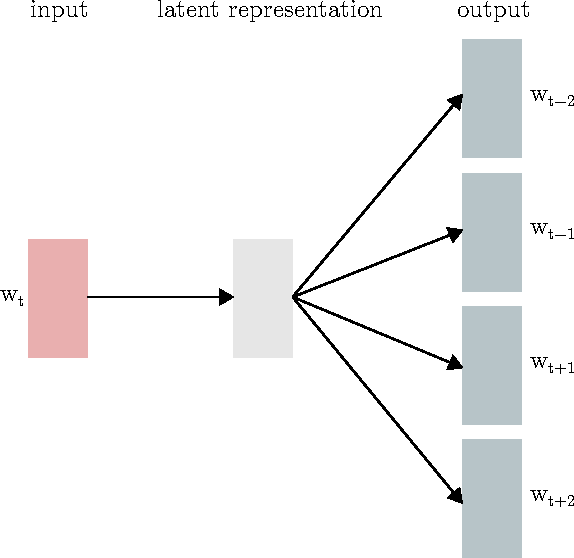
\includegraphics[scale=0.7]{theory/skip-gram-graph}
	\caption{Visualization of the Skip-gram model. Given a single input word it tries to predict the surrounding words. From this the latent representation is learned.}
	\label{fig:theory:skip-gram:graph}
\end{figure}

\subsection{The likelihood function}
The Skip-gram model is optimized by maximum-likelihood. Given a corpus with $\mathcal{D}$ documents where each document have $T_d$ words, the likelihood function is calculated using the conditional probability of observing the surrounding words ($w_{d, t + \ell}$) given the input words ($w_{d, t}\. , t \in [1, T_d]$).
\begin{equation}
\prod_{d = 1}^{\mathcal{D}} \prod_{t = 1}^{T_d} \prod_{\ell} p(w_{d, t + \ell} | w_{d, t})
\label{eq:theory:skipgram:full-likelihood}
\end{equation}

The details about which document there currently is used, are typically omitted from the expressions. Thus equation \eqref{eq:theory:skipgram:full-likelihood} becomes:
\begin{equation}
\prod_{t = 1}^{T} \prod_{\ell} p(w_{t + \ell} | w_{t})
\end{equation}

Since words closer to $w_t$ are expected to be more related to that word, the near surrounding words are weighed higher. This is not modelled by explicit weights, but instead by letting $\ell \in [-R, R] \setminus \{ 0 \}$ where $R \sim U[1, C]$ \cite{word2vec-comparing}.

As usual the negative log is used to get the loss function:
\begin{equation}
\mathcal{L} = - \sum_{t = 1}^T \sum_{\ell} \ln( p(w_{t + \ell} | w_t) )
\end{equation}

In \cite{word2vec-details} a likelihood function is used (sign is flipped), and it is averaged over time ($\sfrac{1}{T}$ is multiplied).

\subsection{Forward pass}
The conditional probability $p(w_{t + \ell} | w_t)$ is calculated using a log-linear model. This is best explained by considering a neural network, with a single hidden layer and no non-linear units ($\theta(a) = a$).

\begin{figure}[H]
	\centering
	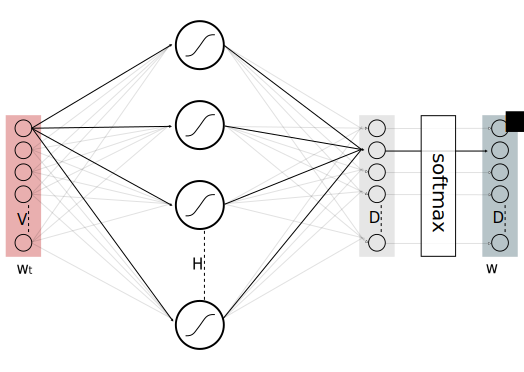
\includegraphics[scale=0.7]{theory/skip-gram-network}
	\caption{Visualization of a single pass though the Skip-gram network.}
	\label{fig:theory:skipgram:network}
\end{figure}

As seen in Figure \ref{fig:theory:skipgram:network} the Skip-gram model is really just a very simple feed forward neural network. The forward equations for this kind of network have already been covered in section \ref{sec:theory:ffnn}, thus deriving the forward equation for the Skip-gram model is just a simple exercise of using that theory. 

By setting $h_0 = K = V$, $h_1 = D$ and defining $x^t$ as the indicator vector for the word $w_t$, the forward pass becomes:
\begin{equation}
\begin{aligned}
b_{h_1}^t = a_{h_1}^t &= \sum_{i = 1}^V w_{i, h_1} x_i^t, && \forall h_1 \in [1, D] \\
a_{k}^t = a_{h_2}^t &= \sum_{h_1 = 1}^{D} w_{h_1, h_2} b_{h_1}^t, && \forall h_2 \in [1, V] \\
y_k^t &= \frac{\exp(a_k^t)}{\sum_{k'=1}^V \exp(a_{k'}^t)}, && \forall k \in [1, V]
\end{aligned}
\label{eq:theory:skipgram:forwardpass}
\end{equation}

It is possible to reformulate the \eqref{eq:theory:skipgram:forwardpass} equations, such that they appear as in \cite{word2vec-details}. However it is a bit convoluted as it requires using vector notation and using the fact that $\mathbf{x}_{w_t}$ is an indicator vector to do subscript selection. Thus that won't be covered here, but see Appendix \ref{appendix:skipgram} for how it can be done.

This calculation of $y_k^t$ is problematic since it contains a sum over all words in the vocabulary. In the Skip-gram model the vocabulary can be of size $10^5$ to $10^7$ \cite{word2vec-details}. This is why \cite{word2vec-comparing, word2vec-details, word2vec-explained} uses an approximation in form of either \textit{hierarchical softmax} or \textit{negative-sampling}. These approximations will not be discussed here, but are worth considering as they will reduce the computational complexity from $\mathcal{O}(V)$ to $\mathcal{O}(\ln_2(V))$ \cite{word2vec-comparing}.

\subsection{Backward pass}

Deriving the backward pass have similarly been covered in section \ref{sec:theory:ffnn}. First step is to express $\ln( p(w_{t + \ell} | w_t) )$ using a target vector, this vector will be denoted $t^{t+\ell}$ for the word $w_{t + \ell}$:
\begin{equation}
\mathcal{L} =  - \sum_{t = 1}^T \sum_{\ell} \ln( p(w_{t + \ell} | w_t)) =  - \sum_{t = 1}^T \sum_{\ell} \sum_{k=1}^V t_k^{t+\ell} \ln(y_k^t)
\end{equation}

This loss function is a little difference compared to that in section \ref{sec:theory:ffnn}. However because it maintains a linear relation to the loss function used in section \ref{sec:theory:ffnn}, this dosen't matter.
\begin{equation}
\begin{aligned}
\frac{\partial \mathcal{L}}{\partial w_{h_{\ell-1}, h_\ell}} = \sum_{t = 1}^T \sum_{\ell} \frac{\partial}{\partial w_{h_{\ell-1}, h_\ell}} \left(- \sum_{k=1}^V t_k^{t+\ell} \ln(y_k^t)\right), && \forall \ell \in [1, L + 1]
\end{aligned}
\end{equation}

Now it is just a matters of using the method covered in section \ref{sec:theory:ffnn}. First the $\delta_{h_\ell}$ values are calculated, to denote the time and lag a superscript is added:
\begin{equation}
\begin{aligned}
\delta_{h_1}^{t, t + \ell} &= \sum_{h_2=1}^{H_2} \delta_{h_2}^{t, t + \ell} w_{h_1, h_2}, && h_1 \in [1, D] \\
\delta_{h_2}^{t, t + \ell} = \delta_{k}^{t, t + \ell} &= y_k^t - t_k^{t+\ell}, && k \in [1, V]
\end{aligned}
\end{equation}

After the $\delta_{h_\ell}^{t, t+\ell}$ values are calculated, the weight derivatives can be calculated:
\begin{equation}
\begin{aligned}
\frac{\partial \mathcal{L}}{\partial w_{h_{0}, h_1}}= \sum_{t = 1}^T \sum_{\ell} \delta_{h_1}^{t, t + \ell} x_{h_0}^t, && \forall h_0 \in [1, V], h_1 \in [1, D] \\
\frac{\partial \mathcal{L}}{\partial w_{h_{1}, h_2}}= \sum_{t = 1}^T \sum_{\ell} \delta_{h_2}^{t, t + \ell} b_{h_1}^t, && \forall h_1 \in [1, D], h_2 \in [1, V]
\end{aligned}
\end{equation}

\subsection{From words to sentenses}
The Skip-gram model only directly allows to get a vector representation of a single word, not a sentence or more. However to find a vector representation for a news article one must work on a sentence level. A simple approach is to just take the avenge vector sum of all the words in the article title and perhaps the subhead.

\cleartorecto
%!TEX root = ../Thesis.tex
\chapter{Results}

\section{Software and implementation}
This section will not discuss the details of the model implementations, but will just citrate the work required for creating the results.

Overall the results was generated with the programing language Python \cite{python}. The skip-gram (word2vec) and paragraph2vec (doc2vec) implementation is from the Python module Gensim \cite{gensim}. The Sutskever model \cite{sutskever} have not been made available as an open source module and nobody else have implemented and open sourced it. It was thus necessary to implement a framework for creating the network. For generating fast code, utilizing the GPU and deriving the backward pass, the Theano framework \cite{theano-a, theano-b} was used. From a more thorough discussion on the this implementation please see \autoref{appendix:implementation}.

As the intellectual properties for news articles are typically not addressed to the public domain, no big free corpus of news articles exists. The news articles was thus collected by crawling RSS feeds and using a previously developed heuristic\footnote{\url{https://github.com/AndreasMadsen/article}} for getting the article text and title from the HTML page.

The code for the Sutskever model implementation and generating the results is available under an MIT open source license at \url{https://github.com/AndreasMadsen/bachelor-code}.

\clearpage
%!TEX root = ../Thesis.tex
\section{Skip-gram}

The skip-gram model doesn't need to be trained as there exists a pre trained version at \url{https://code.google.com/p/word2vec/}. This pre trained version has a latent size of 300 dimensions. The weights are trained using the Google News dataset, which is about 100 billion words and unfortunately not publicly available.

The document vectors are then constructed by taking the average sum over all the word vectors. Using the full text of each article is unlikely to provide any good results, as there would be a lot of irrelevant words which would create a lot of noise. 

Instead just the title of the article is used and as an experiment the title and the subhead is also considered.

\paragraph{Document vectors} Using principal component analysis the vector representations of all the documents can be visualized in both cases.
\begin{figure}[H]
	\centering
	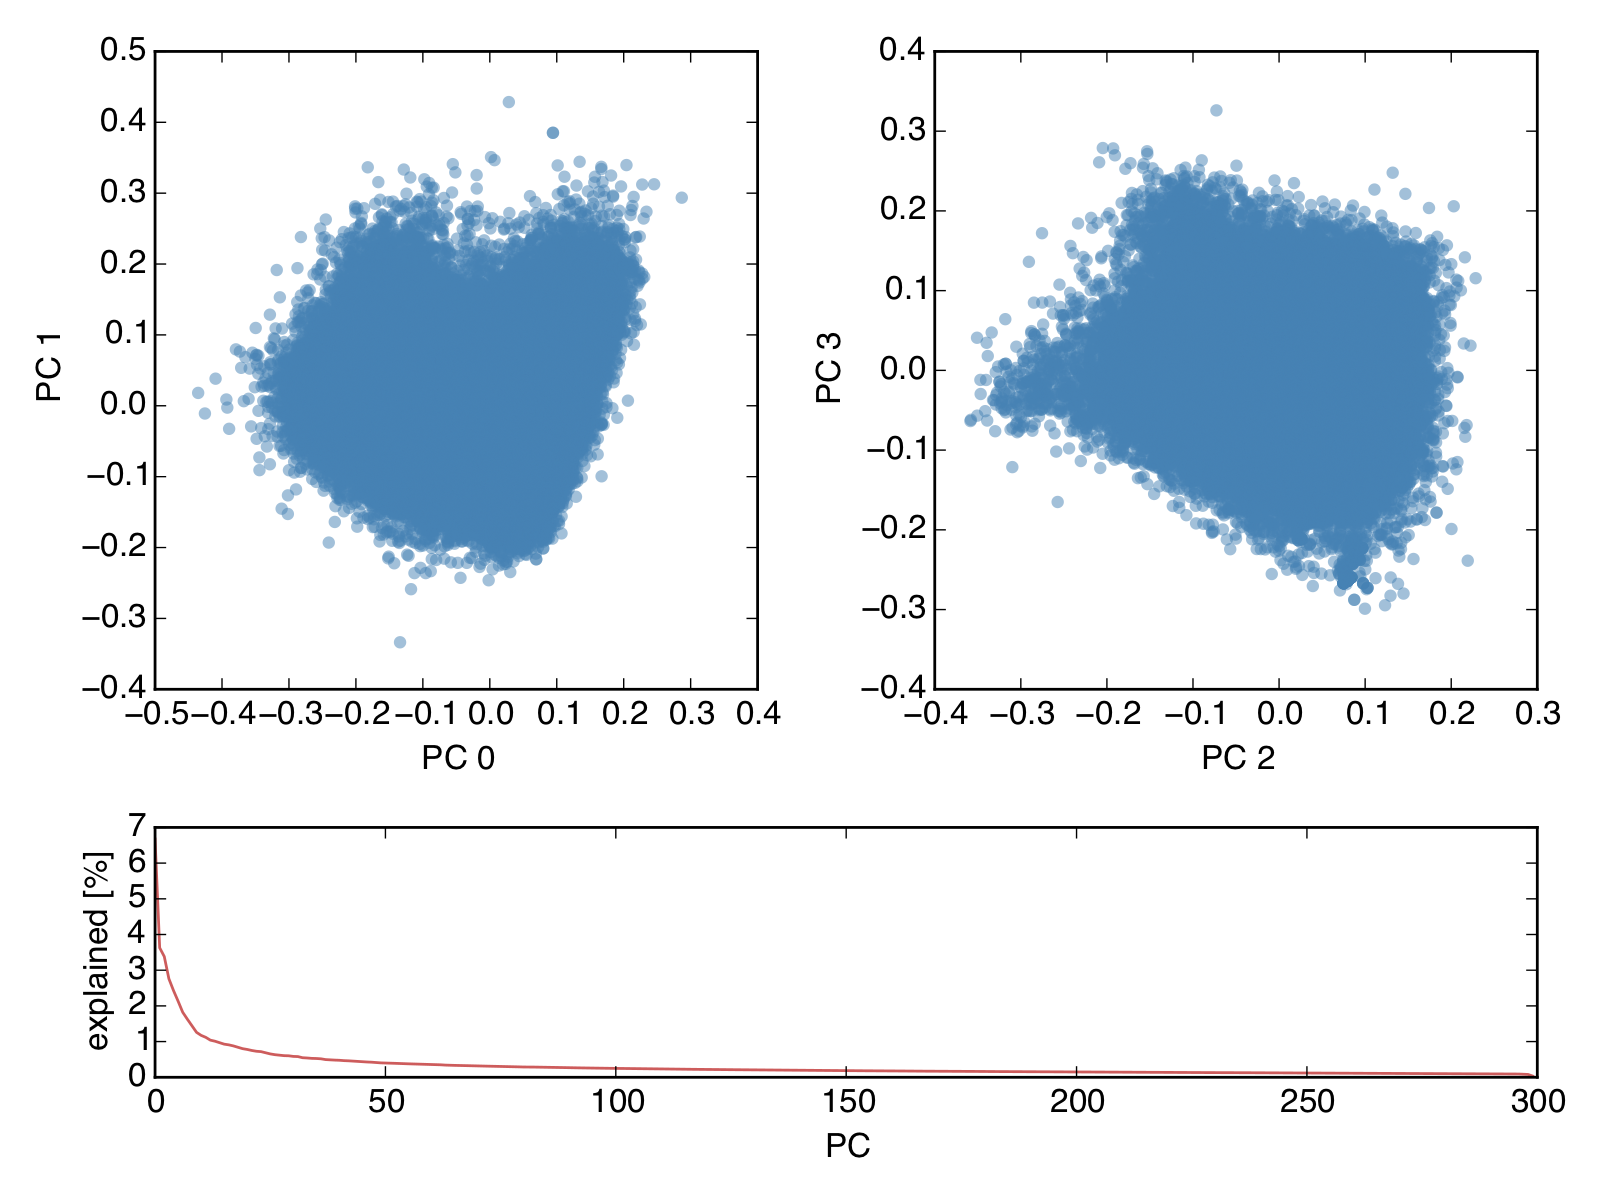
\includegraphics[width=0.9\textwidth]{results/word2vec-title-pca}
	\caption{Document vectors calculated from just the title. Explaned variance on the first 4 principal components is 16.4\%.}
\end{figure}

\begin{figure}[H]
	\centering
	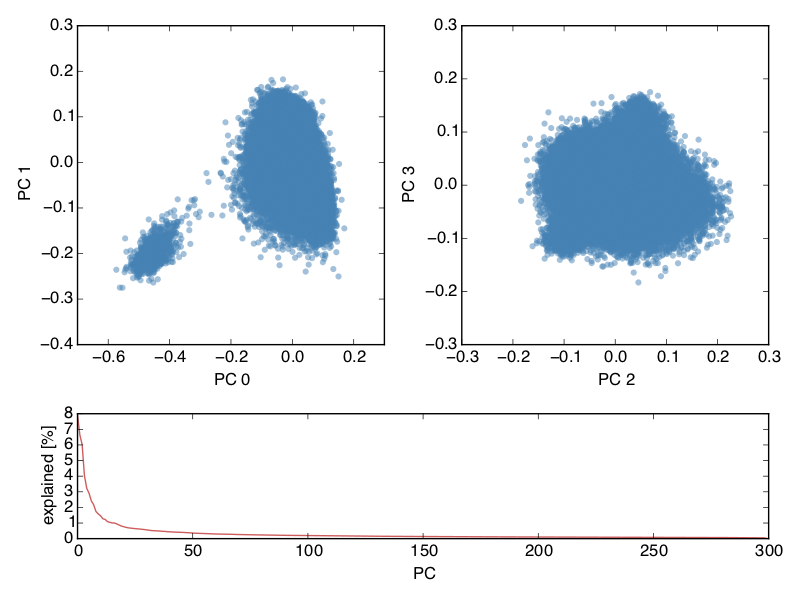
\includegraphics[width=0.9\textwidth]{results/word2vec-both-pca}
	\caption{Document vectors calculated from both title and subhead. Explaned variance on the first 4 principal components is 24.6\%.}
\end{figure}

Without any labeling of the documents the scatter plots are not very informative. The explained variance score is not very high compared to what one usually observes on raw data. This indicated the skip-gram model is somewhat effective in generating descriptive document vectors there aren't too correlated.

An interesting result is that the first principal component seams to contain two big clusters of documents. However by inspecting some of the nodes there do not appear to be any reason for this seperation.

\paragraph{Distance histogram} Since a distance measure will be used to perform the clustering, it makes sense to inspect the histogram of the distance measures. Note that only distances between nodes there are connected by the chronological connectivity matrix have been calculated.

The density estimation required for showing the histogram, also serves the purpose of providing the basis for calculating a somewhat consistent threshold across the diffrent experiments. The threshold $t$ is chosen a the $0.1 \%$ percentile, that is $P(distance < t) = 0.001$. This percentile was chosen qualitatively by running a few experiments, but it turns out it doesn't matter much, as the threshold is not the bottleneck of the performance.

\begin{figure}[H]
        \centering
        \begin{subfigure}[b]{0.49\textwidth}
                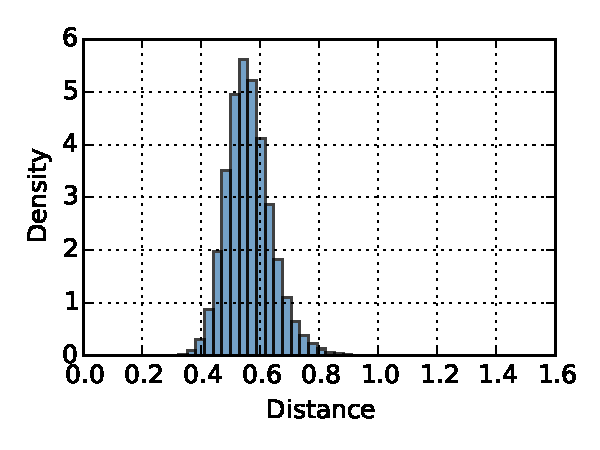
\includegraphics[width=\textwidth]{results/word2vec-title-l2-histogram}
                \caption{Euclidian distance ($t \approx 0.35$)}
        \end{subfigure}
        \begin{subfigure}[b]{0.49\textwidth}
                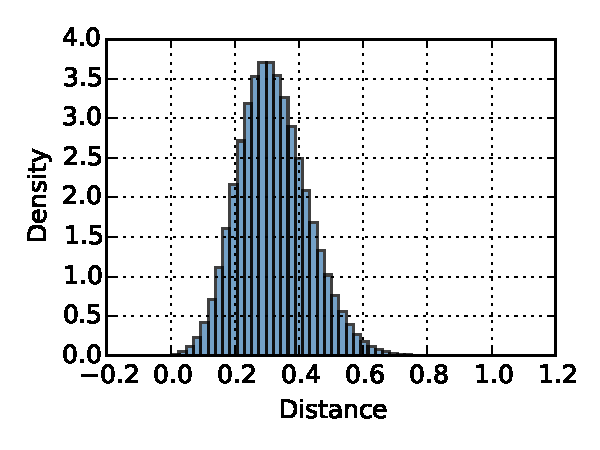
\includegraphics[width=\textwidth]{results/word2vec-title-cos-histogram}
                \caption{Cosine similarity ($t \approx 0.14$)}
        \end{subfigure}
        \caption{Histograms of the distance values using just the title for generating document vectors.}
\end{figure}
\begin{figure}[H]
        \centering
        \begin{subfigure}[b]{0.49\textwidth}
                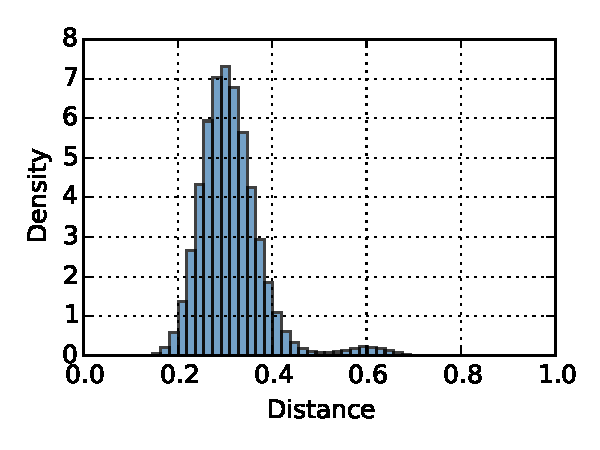
\includegraphics[width=\textwidth]{results/word2vec-both-l2-histogram}
                \caption{Euclidian distance ($t \approx 0.14$)}
        \end{subfigure}
        \begin{subfigure}[b]{0.49\textwidth}
                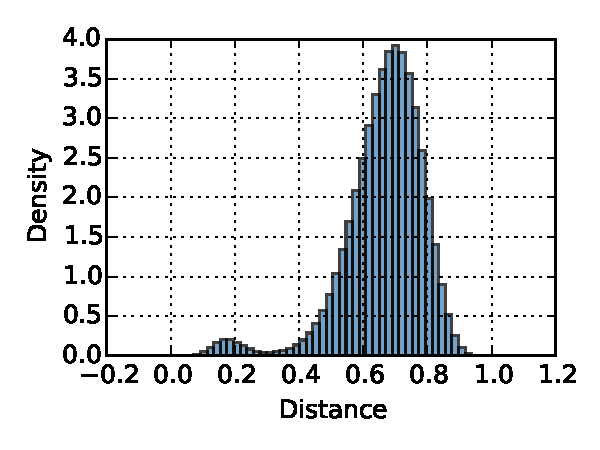
\includegraphics[width=\textwidth]{results/word2vec-both-cos-histogram}
                \caption{Cosine similarity ($t \approx 0.092$)}
        \end{subfigure}
        \caption{Histograms of the distance values using both title and subhead for generating document vectors.}
\end{figure}

The histograms shows the distances are approximately normally distributed. This is not very surprising as the both the euclidian distance and cosine similarly involves a large sum and thus have relations to the central limit theorem.

\paragraph{Inspecting clusters}  None of the 4 variations gives particularly good results. They all cluster the documents such that there is a ridiculously huge amount of unique articles. This alone could indicate the threshold is too small. However simultaneously they all have cluster really big clusters, with up to $31478$ documents in one case. Because there exists clusters that either way to big or way to small, the threshold is not the problem. It is the skip-gram model or perhaps the clustering method there causes the bad results.

\begin{table}[H]
\centering
\begin{tabular}{r|l l l l l l }
size & 1 & 2 & 81 & 318 & 715 & 17023 \\ \hline
amount & 81857 & 3 & 1 & 1 & 1 & 1
\end{tabular}
\caption{Example of the cluster size distribution. In this case both title and subhead was used for generating document vectors and cosine similarity was used for clustering. Note that using euclidian distance yields way more reasonably sized clusters.}
\end{table}

It should be noted that some clusters do provide good results:

\begin{table}[H]
\centering
\begin{tabular}{r|p{10cm}}
id & title \\ \hline
 25167 & Teenage stowaway survives five-hour flight hiding in wheel of plane \\
 25354 & Survival of teenage stowaway on five-hour flight to Hawaii is medical 'miracle', say experts \\
 25140 & Teenager stowaway 'survives five-hour flight in wheel of plane' \\
 26276 & How teenage boy stowed away on plane wheel well \\
 25567 & Teenage stowaway survives five-hour flight in jet's wheel
\end{tabular}
\caption{A cluster containing articles about the same storry. Produced using euclidian distance on document vectors produced from both title and subhead.}
\end{table}
 
Similar results can be found when just looking at the title and using euclidian distance for clustering. However using cosine similarity did not yield any meaningful results, independent of whether or not the subhead was included. This is wired as the skip-gram papers \cite{word2vec-comparing, word2vec-details} uses the cosine similarity for finding similar words. It could be because cosine similarity is usually used in a context where the length of the vector isn't important. But in this case having a big length could indicate how extreme the article is in its language, which could be created to the story. 

\clearpage
%!TEX root = ../Thesis.tex
\section{Paragraph2vec}

The pre trained skip-gram model can't be used as basis for training the paragraph2vec model, as it don't contain the weights used in the hierarchical softmax, nor does it contain the structure of the Hoffman tree. Because of this both word and document vectors was trained using the gensim implementation.

The model was trained using the full text of all 273813 articles. The dimensionality of the word and document vectors was set to 500. Furthermore the model was trained over 10 epochs, with an initial learning rate of 0.025, which then decreased with 0.002 for each epoch. The vector representations of the chronologically first 100000 articles was then extracted from the final model.

Note that gensim doesn't provide any way of inspecting the loss function directly which is why no such curve is shown here.

\paragraph{Document vectors} Using principal component analysis the vector representations of all the documents can be visualized in both cases.

\begin{figure}[H]
	\centering
	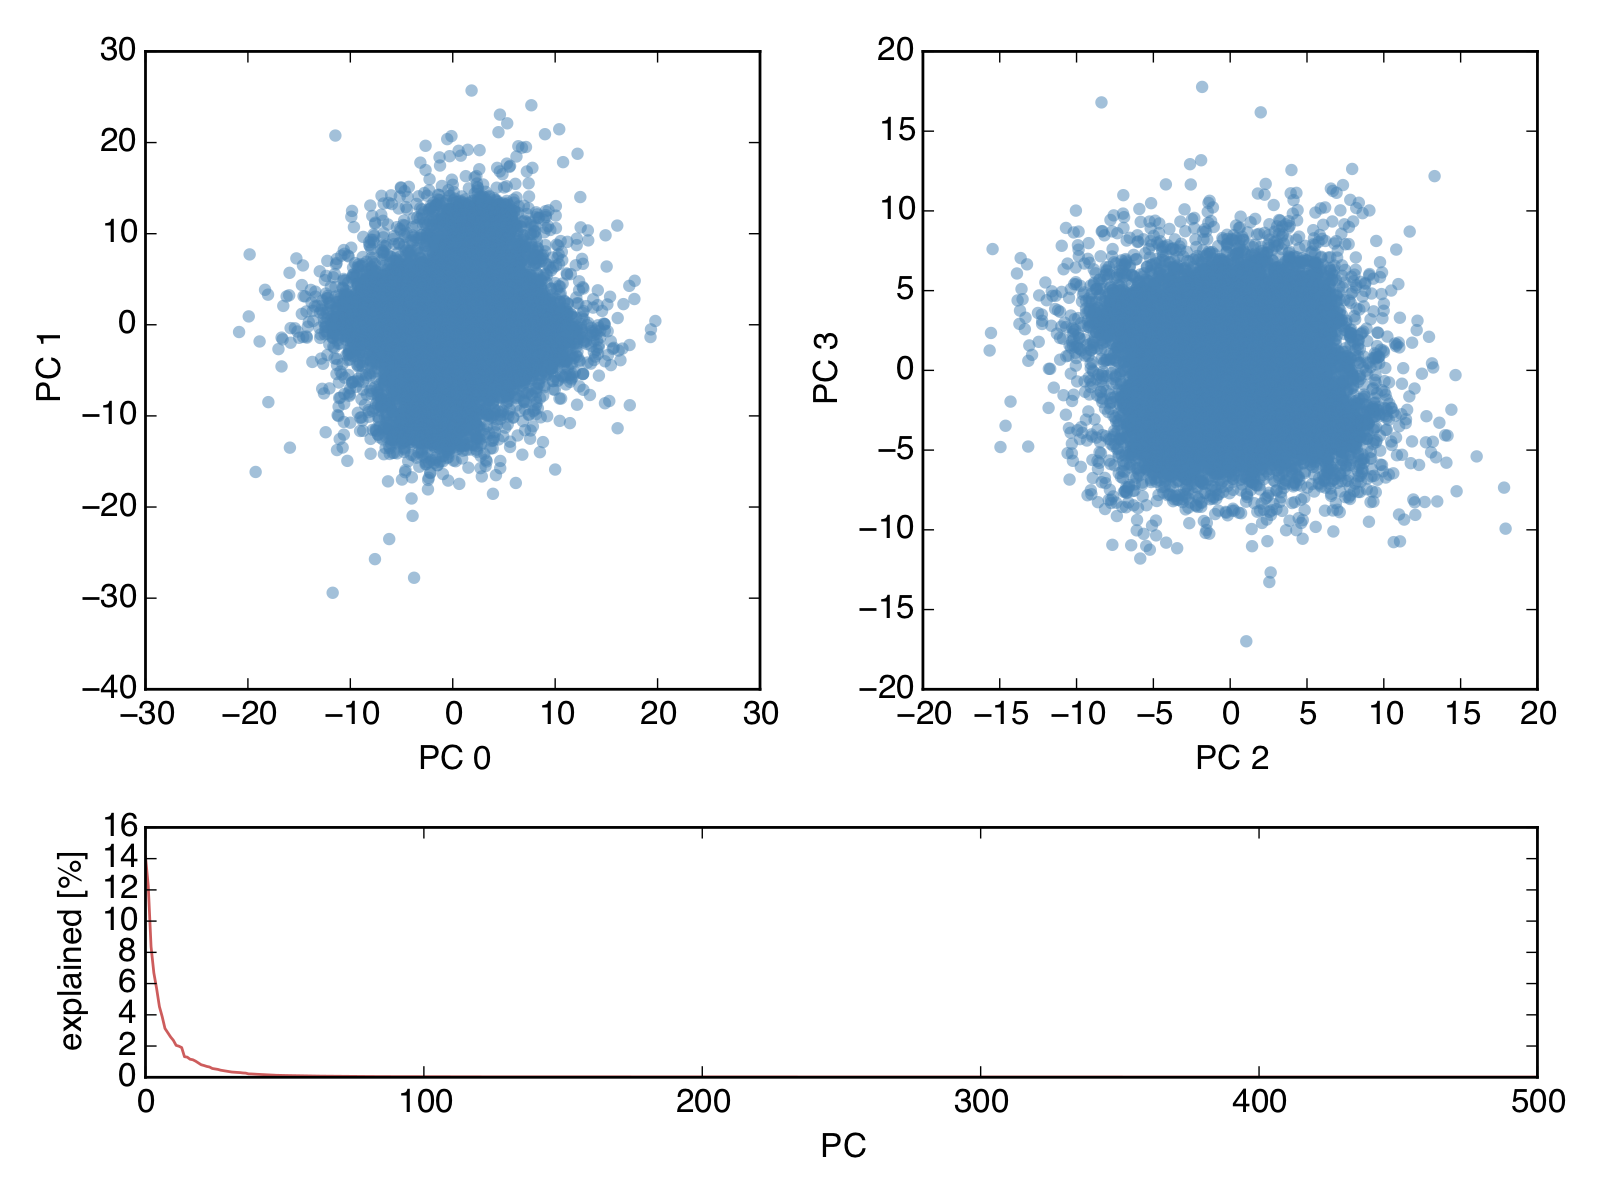
\includegraphics[width=0.9\textwidth]{results/doc2vec-pca}
	\caption{Document vectors calculated from just the title. Explained variance on the first 4 principal components is 41.4\%.}
\end{figure}

The explained variance is 41.4\% for the first 4 principal components, which may be higher than expected. This might be because word2vec part of the model, is quite good at guessing a missing word given just a short context. The big context which is what the document vector provides, may not be very important and only inform about the general rhetorical pattern. This could be (formal versus informal) or (angry versus happy). There thus exists a lower dimensional space there contains almost the same information as the 500 dimensional space.

\paragraph{Distance histogram} Again because the distance is used for clustering, the distance histogram is inspected. Furthermore the $0.1\%$ percentile is used for calculating the threshold $t$.

\begin{figure}[H]
        \centering
        \begin{subfigure}[b]{0.49\textwidth}
                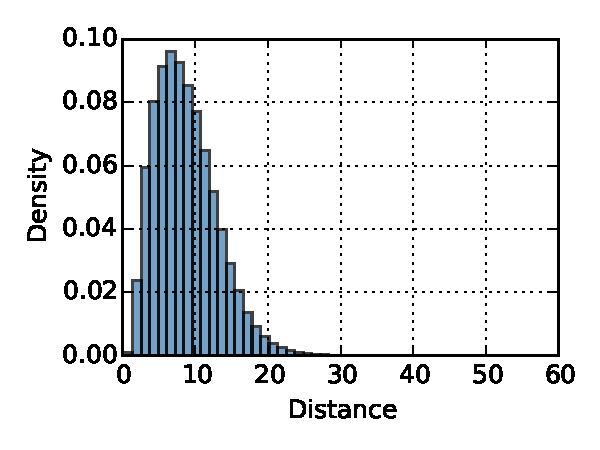
\includegraphics[width=\textwidth]{results/doc2vec-l2-histogram}
                \caption{Euclidean distance ($t \approx 1.35$)}
        \end{subfigure}
        \begin{subfigure}[b]{0.49\textwidth}
                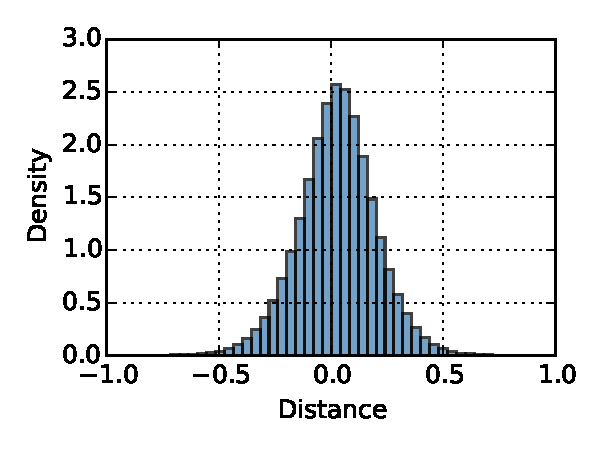
\includegraphics[width=\textwidth]{results/doc2vec-cos-histogram}
                \caption{Cosine similarity ($t \approx -0.66$)}
        \end{subfigure}
        \caption{Histograms of the distance between the document vectors.}
\end{figure}

The distance histograms are distribution wise a bit cleaner than in the skip-gram case. This is likely because the distribution of the document is more multivariate normal, at least when inspecting the PCA plots. This will of cause result a cleaner distribution in the distance as well.

The euclidean distance distribution looks like a gamma or $\chi^2$ distribution. This is likely because of the squaring in the distance calculation, which prevents the distance from becoming negative. In the skip-gram case this was less of an issue because the mean (relative to the standard deviance) was larger.

\paragraph{Inspecting clusters} From inspecting the clusters the result seem to be worse when comparing to the skip-gram case.

When inspecting the cluster distribution it turns out that with paragraph2vec, clustering with cosine similarity actually yields more reasonably sized clusters, compared to when the euclidean distance is used for clustering. This may be because of the $\chi^2$ like distribution of the euclidean distances, which makes it more difficult to separate articles about the same story from those about different stories. It's possible that a more fine-tuned threshold could yield better results, but in any case there still exists too small and way too big clusters.

\begin{table}[H]
\centering
\begin{tabular}{r|l l l l l l l }
size & 1 & 2 & 3 & 421 & 711 & 1855 & 3326 \\ \hline
amount & 93665 & 8 & 2 & 1 & 1 & 1 & 1
\end{tabular}
\caption{The cluster distribution using an euclidean distance shows unreasonably large and small clusters, and no reasonably or few reasonably sized clusters.}
\end{table}

Unfortunately the actual clusters that the clustering algorithm produces when using cosine similarity don't appear to capture any specific story. This is possibly because the document vectors only captures the overall mood of the article. For example the cluster in Table \ref{table:paragraph2vec:example} shows articles related to different bad events.

At last it was checked if the ``teenage stowaway'' cluster existed in this case. This should be a fairly easy set of article to cluster as it contains very specific word combinations. Unfortunately it didn't exists as a single cluster, which again indicates the document vectors only tells about the overall mood of the document, as a way of adjusting the word probabilities.

\begin{table}[H]
\centering
\begin{tabular}{r|p{10cm}}
id & title \\ \hline
  9489 & Ukraine crisis: Draft document reveals sanctions against Russian and Crimean officials \\
  6644 & Six Nations 2014: Stuart Lancaster hints at unchanged England \\
  7573 & US opens emergency oil stockpile in signal to Putin \\
  8998 & Saudi Arabia bans 50 ‘blasphemous’ and ‘inappropriate’ children’s names \\
  7862 & Rangers: Recovery on track after title win - Ally McCoist
\end{tabular}
\caption{Cluster example when using cosine similarity on the paragraph2vec results.}
\label{table:paragraph2vec:example}
\end{table}

\clearpage
%!TEX root = ../Thesis.tex
\section{Sutskever}

As no neural network framework exists for creating networks like the sutskever model, such a framework was written as a part of this thesis. This is a big task where a lot can go wrong, so the first part of this section will attempt to validate the model by having it solve some simple problems.

\subsection{Constructed problems}

Inspired from the learning to execute paper \cite{learning-to-execute} a copy problem is used to validate the model. The idea is simple generate a sequence of random integers between 1 and 9 of length 8 and append an \texttt{<EOS>} element (encoded 0) to that sequence. 
\begin{figure}[H]
\begin{equation*}
\begin{aligned}
[3, 4, 8, 5, 9, 9, 4, 4, 0] \\
[2, 5, 9, 7, 6, 2, 1, 5, 0] \\
[1, 6, 7, 4, 4, 1, 6, 4, 0]
\end{aligned}
\end{equation*}
\caption{Example of integer sequences used in the \textit{copy} problem.}
\end{figure}

Each element of value $i$ is then transformed into an indicator vector, such that the 1-element is at position $i$. The indicator vector will be denoted by a bold font.

Now consider the following three variations of the same problem. Note that that only the \textit{full network} model is required and used for the immediate validation. But the \textit{encoder} and \textit{decoder} problems becomes useful in a detailed analysis.

\paragraph{Full network} To validate the full network the sequence of indicator vectors is used both as input and output. Example: $[\mathbf{3}, \mathbf{4}, \mathbf{8}, \mathbf{5}, \mathbf{9}, \mathbf{9}, \mathbf{4}, \mathbf{4}, \mathbf{0}] \rightarrow [\mathbf{3}, \mathbf{4}, \mathbf{8}, \mathbf{5}, \mathbf{9}, \mathbf{9}, \mathbf{4}, \mathbf{4}, \mathbf{0}]$.

\paragraph{Encoder} The encoder problem is a regression problem where the output is the integer sequence expressed as an vector. Note that the \texttt{<EOS>} isn't included and the vector is divided by 9 to fit between $0$ and $1$. It isn't strictly necessary for the output to be within $[0, 1]$, but it makes it easier to compare to the decoder version of this problem. Example: $[\mathbf{3}, \mathbf{4}, \mathbf{8}, \mathbf{5}, \mathbf{9}, \mathbf{9}, \mathbf{4}, \mathbf{4}, \mathbf{0}] \rightarrow [\sfrac{3}{9}, \sfrac{4}{9}, \sfrac{8}{9}, \sfrac{5}{9}, \sfrac{9}{9}, \sfrac{9}{9}, \sfrac{4}{9}, \sfrac{4}{9}]$.

\paragraph{Decoder} Finally one can consider a decoder version of the \textit{copy} problem. Here the input should be between $0$ and $1$, as this will be used to initial the hidden output $b_{h_1}^{0_d}$ and the cell state $s_{h_1}^{0_d}$. The cell in partially is almost always in the $[0, 1]$ interval. The input and output is the same as in the encoder case, just swapped. Example: $[\sfrac{3}{9}, \sfrac{4}{9}, \sfrac{8}{9}, \sfrac{5}{9}, \sfrac{9}{9}, \sfrac{9}{9}, \sfrac{4}{9}, \sfrac{4}{9}] \rightarrow [\mathbf{3}, \mathbf{4}, \mathbf{8}, \mathbf{5}, \mathbf{9}, \mathbf{9}, \mathbf{4}, \mathbf{4}, \mathbf{0}]$

\subsection{Validateing implementation}

To validate the sutskever model the \textit{full network} version of the \textit{copy} problem was used. The model was configured as:

\begin{table}[H]
\centering
\begin{tabular}{r|c}
	parameter & value \\ \hline
	learning rate ($\eta$) & 0.001 \\
	momentum ($m$) & 0.9 \\
	decay ($\gamma$) & 0.95 \\
	weight initialization & $\mathcal{N}(0, 0.5^2)$ \\
	clipping stratagy & Euclidian \\
	clipping value & 10
\end{tabular}
\caption{Initialization parameters.}
\end{table}

\begin{figure}[H]
	\centering
	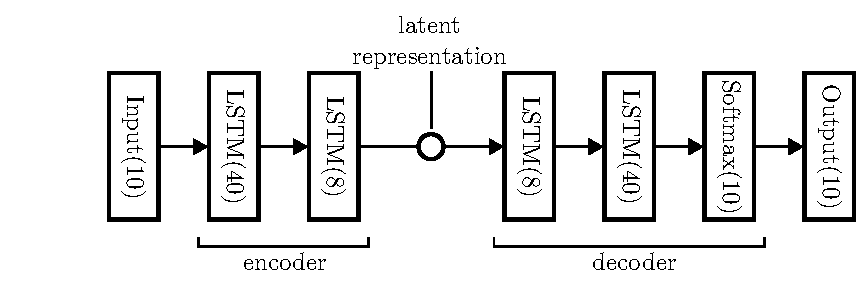
\includegraphics[scale=0.7]{results/sutskever-validate}
	\caption{The arcitecture of the network.}
\end{figure}

The loss curve in Figure \ref{fig:results:sutskever:network-05} shows that the implementation in capable of solving the copy problem and actually converges fairly nicely with a very minimal overfitting.

Whether or not the model solves it such that the encoder solves the \textit{encoder copy} problem and the decoder solves the \textit{decoder copy} is unknown. This is also irrelevant for validating the implementation. However the loss curves are for those two problems are stil shown here in Figure \ref{fig:results:sutskever:decoder-encoder-05} as they will later prove valuable as a reference.

Also note that while solving this problem validates the implementation, it doesn't guarantee an correct implementation, it just makes it very likely that the implementation is correct.

\begin{figure}[h]
	\centering
	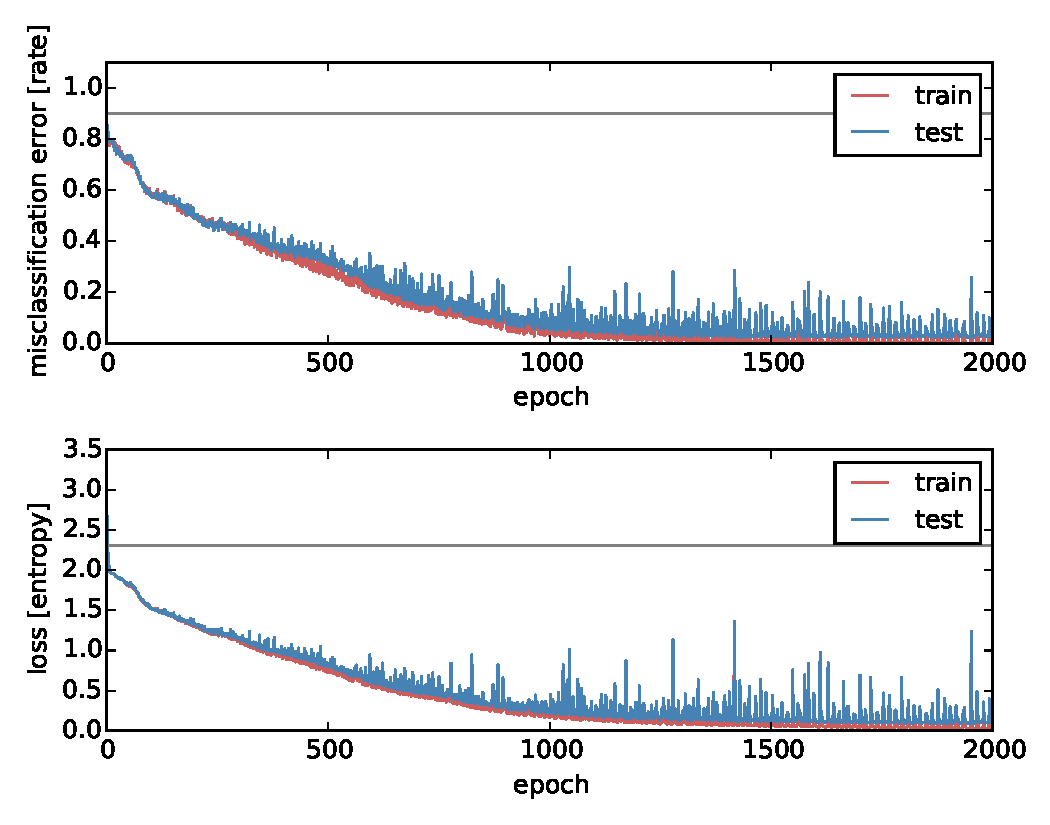
\includegraphics[scale=0.60]{results/sutskever-network-normal-05-rmsgraves}
	\caption{Loss and missclassification rate as a function of the number of epochs on the full sutskever network.}
	\label{fig:results:sutskever:network-05}
\end{figure}
\begin{figure}[H]
        \vspace{-0.5cm}
        \centering
        \begin{subfigure}[b]{0.49\textwidth}
                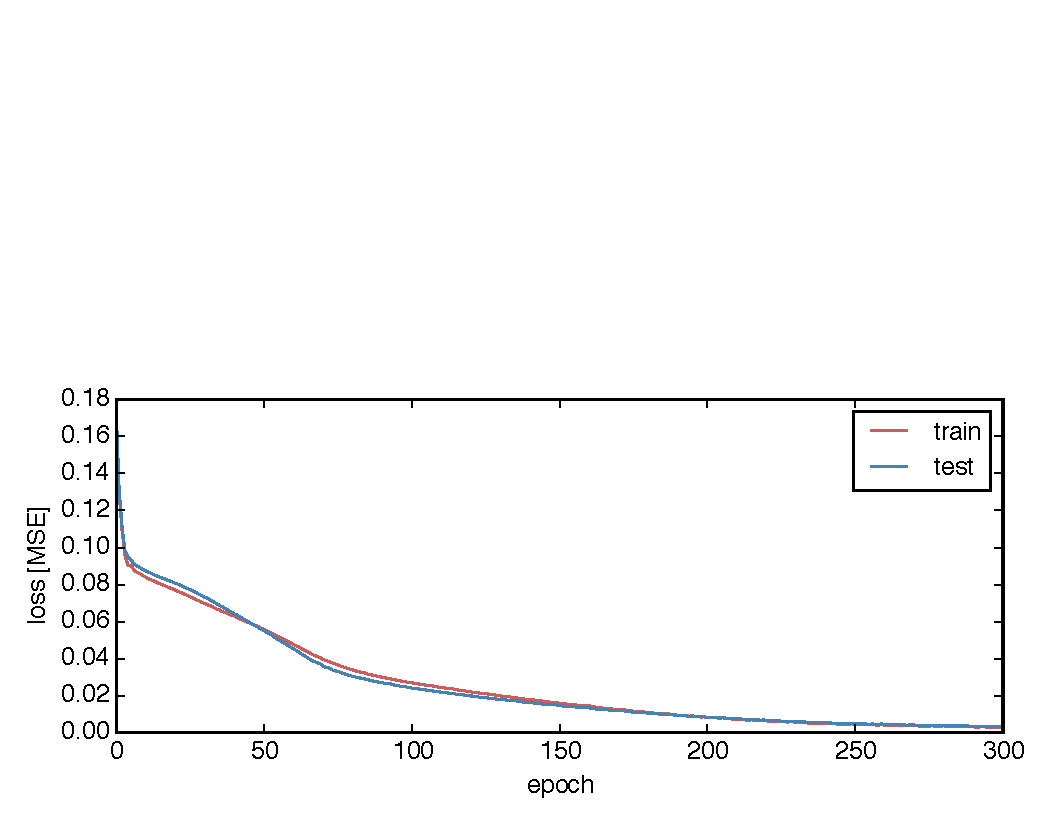
\includegraphics[scale=0.60]{results/sutskever-encoder-normal-05-rmsgraves}
                \caption{Encoder}
        \end{subfigure}
        \begin{subfigure}[b]{0.49\textwidth}
                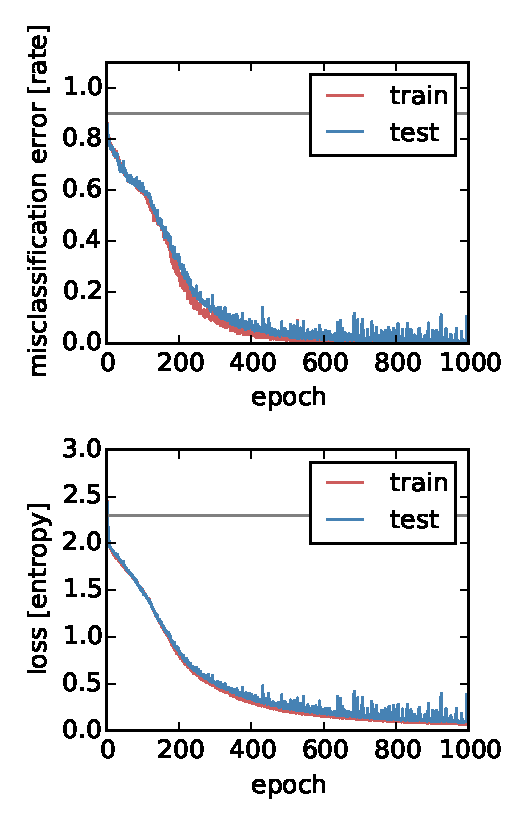
\includegraphics[scale=0.60]{results/sutskever-decoder-normal-05-rmsgraves}
                \caption{Decoder}
        \end{subfigure}
        \caption{Loss and missclassification rate as a function of the number of epochs.}
        \label{fig:results:sutskever:decoder-encoder-05}
\end{figure}

\subsection{Using real data}

Now that the implementation is validated, it can be used on the real problem. The goal is to predict the article title given the subhead, the hope is this should be somewhat similar to the translation problem solved in the original paper \cite{sutskever}. Figure \ref{fig:results:sutskever:example} shows the first 3 observations in the dataset. The entire dataset consists of 273813 news articles, all articles are used for training.

\begin{figure}[H]
\centering
\begin{tabular}{r|p{10cm}}
	title: & Ukrainian President Yanukovych agrees early election \\
	subhead: & Ukrainian President Yanukovych calls an early election, as details emerge of a deal to end political crisis. Ukrainian President Viktor Yanukovych has agreed to an early presidential election as part of a deal to end the long-running crisis.
\end{tabular}
\mbox{}\vspace*{0.5cm}
\begin{tabular}{r|p{10cm}}
	title: & UK floods: Damage 'could have been prevented' \\
	subhead: & Damage during the recent floods could have been prevented if the correct water management techniques had been used, says a group of experts.Some of the damage caused by the recent floods could have been prevented if the correct water management techniques had been used, says a group of leading environmental and planning experts.
\end{tabular}
\mbox{}\vspace*{0.5cm}
\begin{tabular}{r|p{10cm}}
	title: & Five lose housing benefit cut appeal \\
	subhead: & Five disabled social housing tenants lose their Court of Appeal bid to have benefit cuts for those with spare bedrooms ruled unlawful. Five disabled social housing tenants have lost their Court of Appeal bid to have benefit cuts for those with spare bedrooms ruled unlawful.
\end{tabular}
\caption{Three examples on title (target) and input (subhead).}
\label{fig:results:sutskever:example}
\end{figure}

It turns out that using $\mathcal{N}(0, 0.5^2)$ to initialize the weights has such a high variance that the gradients become not-a-number (nan). To solve this $\mathcal{N}(0, 0.1^2)$ is used to initialize the weights, this is also what Alex Graves uses in his book \cite{alexgraves}.

This allows the training to continue for some iterations, to have it to continue for a longer duration with out getting not-a-number gradients the momentum and learning rate is also decreased. The final configuration is shown in Table \ref{fig:results:sutskever:article-parameters} and Figure \ref{fig:results:sutskever:article-artitecture}.
\begin{table}[h]
\centering
\begin{tabular}{r|c}
	parameter & value \\ \hline
	learning rate ($\eta$) & 0.0001 \\
	momentum ($m$) & 0.2 \\
	decay ($\gamma$) & 0.95 \\
	weight initialization & $\mathcal{N}(0, 0.1^2)$ \\
	clipping stratagy & Euclidian \\
	clipping value & 10
\end{tabular}
\caption{Initialization parameters.}
\label{fig:results:sutskever:article-parameters}
\end{table}

\begin{figure}[h]
	\centering
	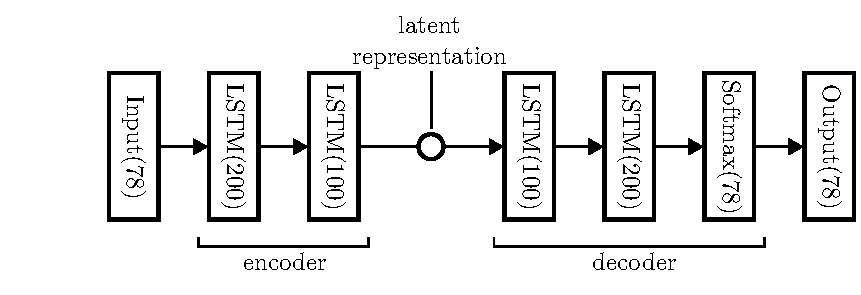
\includegraphics[scale=0.7]{results/sutskever-article}
	\caption{The arcitecture of the network.}
	\label{fig:results:sutskever:article-artitecture}
\end{figure}

\begin{figure}[H]
	\centering
	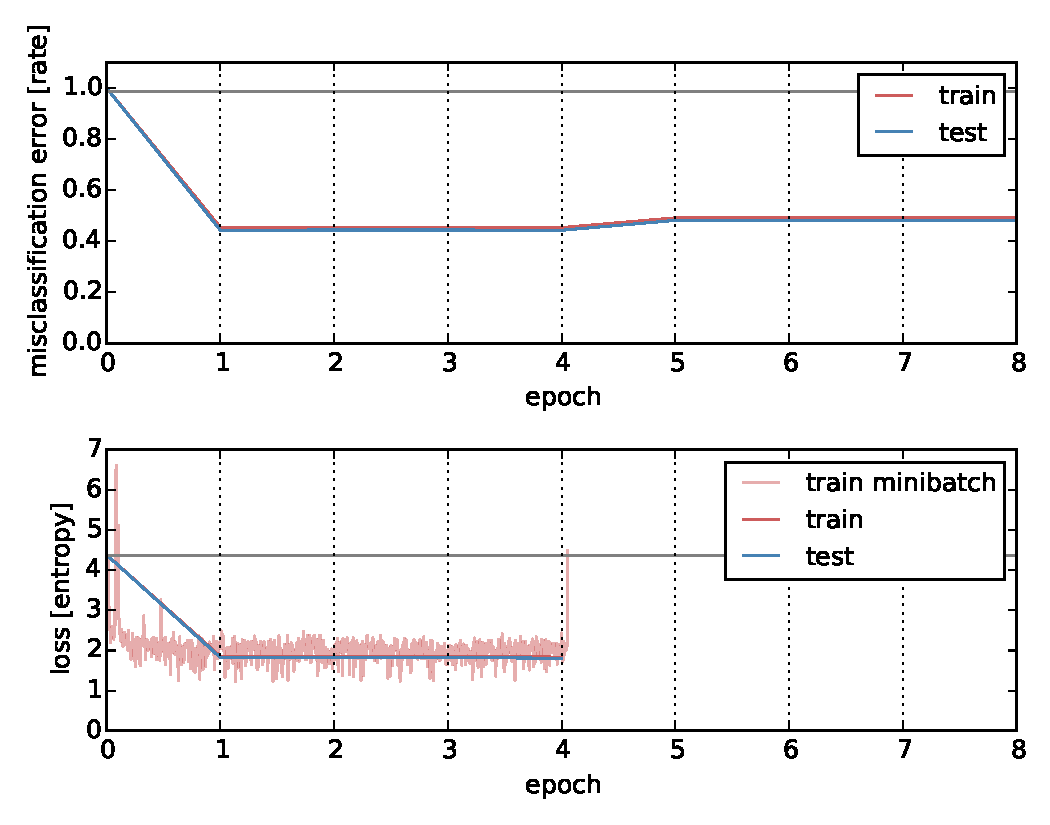
\includegraphics[scale=0.60]{results/sutskever-article-normal-01-rmsgraves-m02.pdf}
	\caption{Loss and missclassification rate as a function of the number of epochs on the full sutskever network.}
	\label{fig:results:sutskever:article-learning}
\end{figure}

Figure \ref{fig:results:sutskever:article-learning} shows that the model didn't converge after 4 epochs. Note that after approximately 4 epochs the gradients became not-a-number. The misclassification rate is only $0.5$ so maybe there could be some meaning in the output. But from inspecting the prediction for the first 3 observations (Se Table \ref{fig:results:sutskever:predictions}) it is clear that isn't the case.
\begin{table}[h]
\centering
\begin{tabular}{p{9cm}|p{2cm}}
	target & prediction \\ \hline
	Ukrainian President Yanukovych agrees early election & \texttt{<EOS>} \\
	UK floods Damage 'could have been prevented' & \texttt{<EOS>} \\
	Five lose housing benefit cut appeal & \texttt{<EOS>}
\end{tabular}
\caption{Target and prediction of the first 3 observations.}
\label{fig:results:sutskever:predictions}
\end{table}

The model just predicts a long sequence of \texttt{<EOS>} which will match a fairly big part of the target, because it padded with \texttt{<EOS>} to fit the longest sequence in that mini-batch.

Each epoch contains 2140 mini-batches and takes about 3 hours to run. The 4 epochs that ran before the gradients became not-a-number thus took 12 hours. This should be enough time to find a better solution than just predicting \texttt{<EOS>}.

\subsection{Diagnosing the problem}

It is possible that the model is just sucked in a local minima. However it turns that decreasing the standard deviance for the weight initialization in the \textit{copy} problem causes similar issues (see Table \ref{fig:results:sutskever:copy-parameters} for the full configuration). In this problem the sequences are all equally long before padding, so just predicting \texttt{<EOS>} isn't a naturally good choice. However the model predictions are still independent of the input and somewhat constant just like in the real data case. For example $[1, 1,1,1, 7, 7, 7, 7, 0]$ is always the prediction given a seed of $42$.

However it turns out that the decoder and encoder themself converges just fine, though it is not as smooth as when $\mathcal{N}(0, 0.5^2)$ is used for weight initialization.
\begin{table}[h]
\centering
\begin{tabular}{r|c}
	parameter & value \\ \hline
	learning rate ($\eta$) & 0.001 \\
	momentum ($m$) & 0.9 \\
	decay ($\gamma$) & 0.95 \\
	weight initialization & $\mathcal{N}(0, 0.1^2)$ \\
	clipping stratagy & Euclidian \\
	clipping value & 10
\end{tabular}
\caption{Initialization parameters for the copy problem with $\sigma = 0.1$.}
\label{fig:results:sutskever:copy-parameters}
\end{table}

\begin{figure}[h]
	\centering
	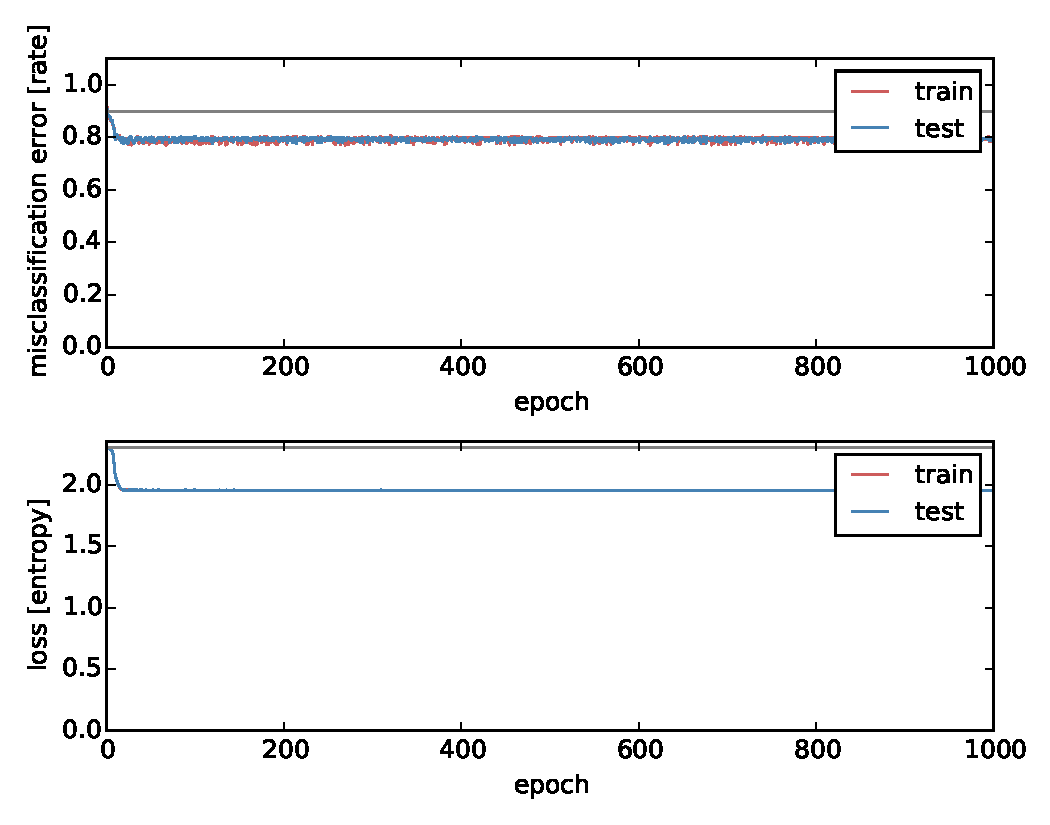
\includegraphics[scale=0.60]{results/sutskever-network-normal-01-rmsgraves}
	\caption{Loss and missclassification rate as a function of the number of epochs on the full sutskever network.}
	\label{fig:results:sutskever:network-01}
\end{figure}
\begin{figure}[H]
        \vspace{-0.5cm}
        \centering
        \begin{subfigure}[b]{0.49\textwidth}
                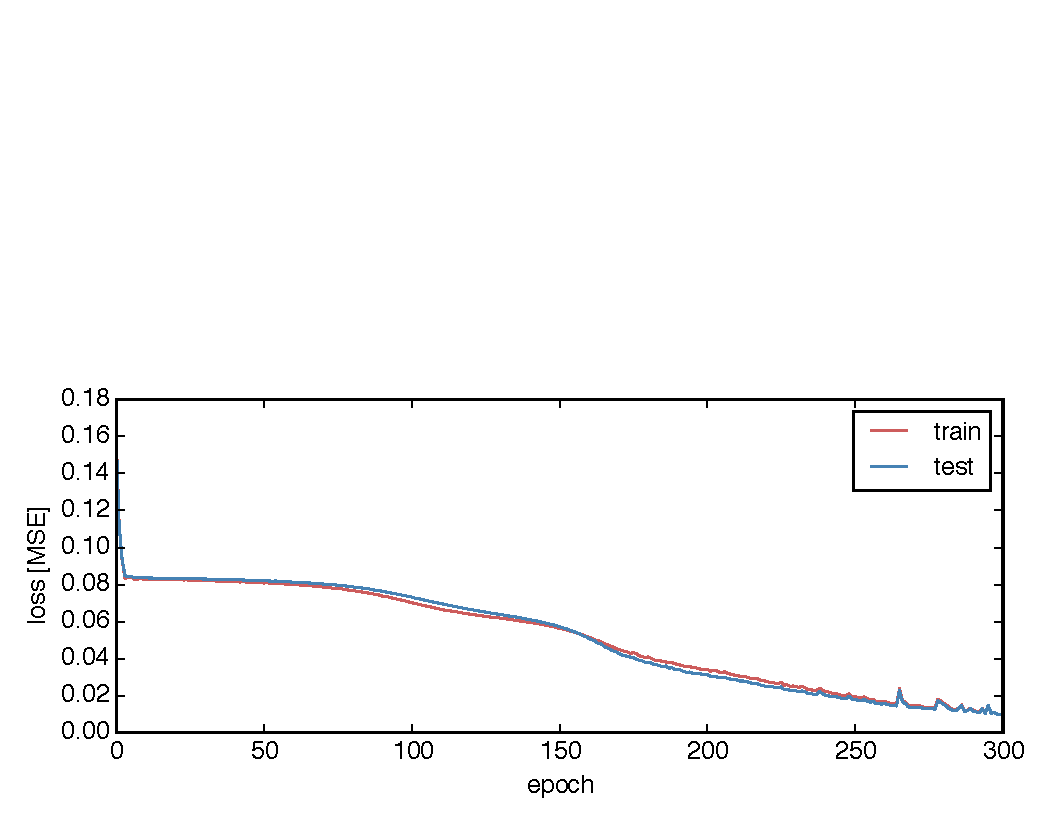
\includegraphics[scale=0.60]{results/sutskever-encoder-normal-01-rmsgraves}
                \caption{Encoder}
        \end{subfigure}
        \begin{subfigure}[b]{0.49\textwidth}
                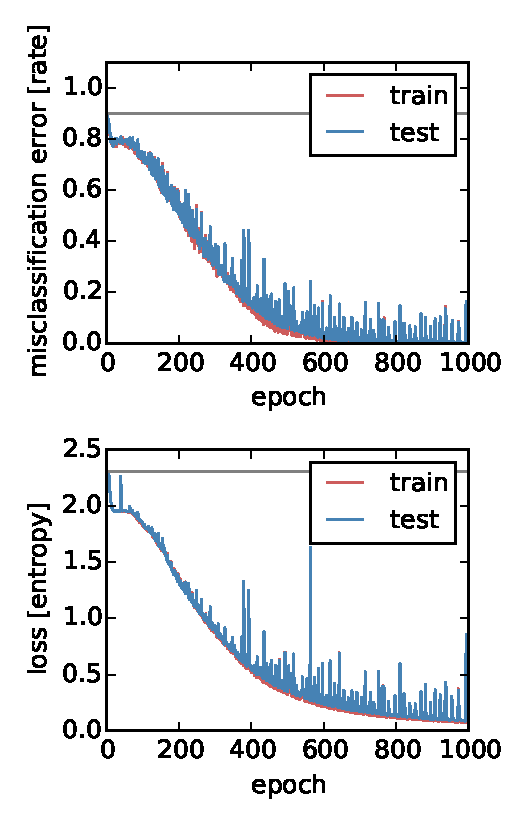
\includegraphics[scale=0.60]{results/sutskever-decoder-normal-01-rmsgraves}
                \caption{Decoder}
        \end{subfigure}
        \caption{Loss and missclassification rate as a function of the number of epochs.}
        \label{fig:results:sutskever:decoder-encoder-01}
\end{figure}

There is a lot of spikes in the encoder and decoder loss curves (Figure \ref{fig:results:sutskever:decoder-encoder-01}) these could properly have been avoided by choosing a smaller \textit{clip} value. Likewise it is entirely possible that some other hyperparameter choices could have caused the full network to converge properly. To investigate that possibility a grid search over the hyperparameters was performed.

\begin{table}[h]
\centering
\begin{tabular}{r|c}
	parameter & value(s) \\ \hline
	learning rate ($\eta$) & [0.0001, 0.001, 0.01, 0.1, 0.2] \\
	momentum ($m$) & [0, 0.2, 0.9] \\
	decay ($\gamma$) & [0.9, 0.95] \\
	weight initialization & $\mathcal{N}(0, 0.1^2)$ \\
	clipping stratagy & Euclidian \\
	clipping value & [1, 5, 10, 50]
\end{tabular}
\caption{Tried parameter combinations for solving the \textit{full network copy} problem.}
\label{table:resutls:sutskever:gridsearch-range}
\end{table}
\begin{table}[h]
\vspace{-0.5cm}
\centering
\begin{tabular}{r|c|c}
	parameter & best & worst  \\ \hline
	learning rate ($\eta$) & 0.01 & 0.1 \\
	momentum ($m$) & 0.9 & 0 \\
	decay ($\gamma$) & 0.9 & 0.9 \\
	weight initialization & $\mathcal{N}(0, 0.1^2)$ & $\mathcal{N}(0, 0.1^2)$ \\
	clipping stratagy & Euclidian & Euclidian \\
	clipping value & 5 & 10
\end{tabular}
\caption{Best and worst choose for hyperparameters, given the gridsearch in Table \ref{table:resutls:sutskever:gridsearch-range}.}
\end{table}

While there are good and bad choices none of them makes the full network converge, as seen in Figure \ref{fig:results:sutskever:gridsearch-clip} and \ref{fig:results:sutskever:gridsearch-momentum}.
\begin{figure}[h]
	\centering
	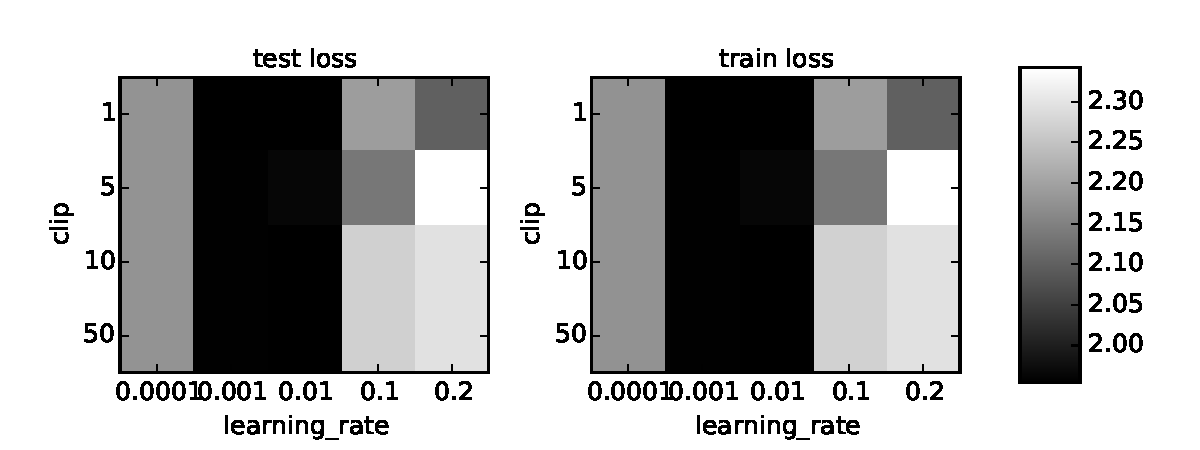
\includegraphics[scale=0.60]{results/sutskever-gridsearch-clip}
	\caption{Gridsearch on learning rate and clip, other parameter variations are meaned out.}
	\label{fig:results:sutskever:gridsearch-clip}
\end{figure}
\begin{figure}[H]
	\centering
	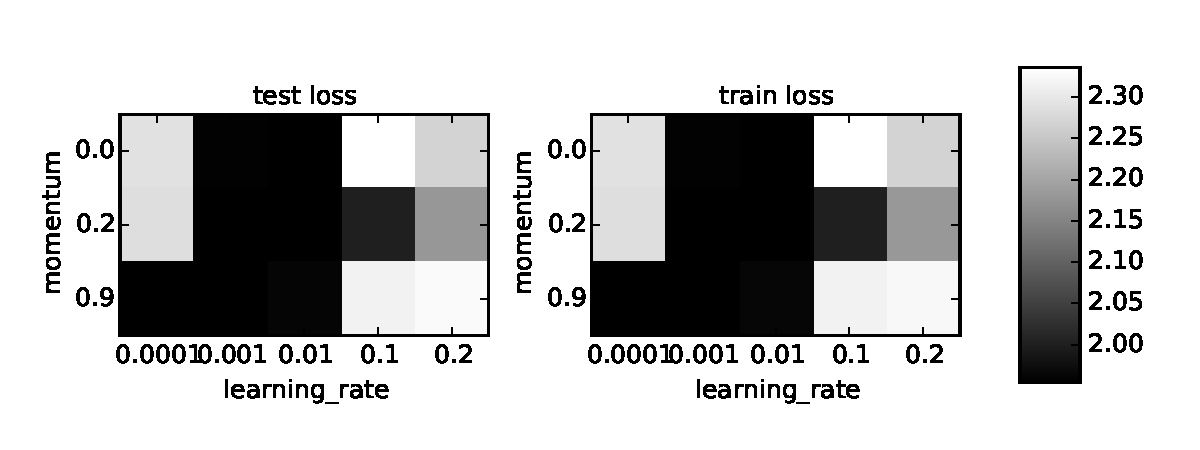
\includegraphics[scale=0.60]{results/sutskever-gridsearch-momentum}
	\caption{Gridsearch on learning rate and momentum, other parameters variations are meaned out.}
	\label{fig:results:sutskever:gridsearch-momentum}
\end{figure}

The encoder and decoder themself can converge and hyperparameter optimization of the full network doesn't work. All this suggests that it is the combination of the many layers and the smaller standard deviance that causes the problem.

\subsection{Vanshing gradient}
It is not unusual that deep networks and small initial weights causes problems. This is because of the vanishing gradient problem. This is particular a problem in recurrent neural networks, because the iteration over the sequence actually causes the network to be much deeper than it appears to be. Using LSTM units solves this to some extent, however having many layers is still an issue. This is best seen by just considering a simple feed forward neural network with many layers and following the $\delta$ calculations.

Because the last layer is a softmax and one can expect and uniform distribution as the initial distribution and the target is often zero, $\delta_{L+1}$ can be approximated as $\frac{1}{10}$ (there are 10 classes). The remaining $\delta$ values are then calculated as:
\begin{equation}
\delta_{h_\ell} = \theta'(a_{h_\ell}) \sum_{h_{\ell+1} = 1}^{H_{\ell+1}} \delta_{h_{\ell+1}} w_{h_\ell, h_{\ell+1}}
\end{equation}

The maximum value of $\theta'(\cdot)$ when $\theta$ is the sigmoid function is approximately $0.23$, and shouldn't expect more than $0.1$ from the weights. One then gets:
\begin{equation}
\delta_{h_L} \approx 0.23 \sum_{h_{\ell+1} = 1}^{H_{\ell+1}} \frac{1}{10} \cdot 0.1 \lesssim \delta_{h_{L+1}} \approx \frac{1}{10}
\end{equation}

The $\delta_{h_\ell}$ will thus decrease for each layer causing the gradients for the bottom layers to be near zero.

Note that because the size of $\delta_{h_\ell}$ depends on $H_{\ell+1}$, one could use different standard deviance values depending on the $H_{\ell+1}$ value for each layer. This was attempted and didn't work, though more experiments could have been done. Another solution is to use rectified linear unit (ReLU) as the activation function which as been shown not to suffer from the vanishing gradient problem, due to the lack of time this was not attempted.



%!TEX root = ../Thesis.tex
\chapter{Conclusion}

In this thesis 3 models for creating document vectors have been analyzed for the purpose of clustering articles related to the same story. While this is a very specific application the performance of the models will be related to their ability to create good vector representations of documents.

\paragraph{Skip-gram} The skip-gram model which is the most primitive and oldest of the three model, actually turned out to produce surprisingly good document vectors. It is not that the document vector are amazing and solves the problem well, but given that the purpose of the skip-gram model is to find good word vectors and not document vectors the good performance is surprisingly good. It is possible that a more clever weighted sum could have improved the result further, for example weighs nouns higher. But as the paragraph2vec paper \cite{doc2vec} also states the performance will always be limited by the fact that the purpose of the model is to find word vectors not document vectors.

\paragraph{paragraph2vec} While the skip-gram model was surprisingly good the paragraph2vec was surprisingly bad. According to the paragraph2vec paper \cite{doc2vec} this model should be better than the usual bag-of-word models and should produce a much better document vector than just taking the mean of the word vectors. Unfortunately this does not seams to be the case. A possible explantation is that the document vectors that the model produces doesn't represent the semantic meaning very well but rather the mood or political point of view of the document. The reasoning here is that semantic meaning is likely found the short context which is may best be predicted by the surrounding words, while the mood is found in the larger context which is where the document vectors help in the prediction. It is also entirely possible that the model work better with short documents like sentences and using the full article text isn't the optimal choice. While that is said the paragraph2vec paper \cite{doc2vec} does claim to work on documents of any length. The effect of the document length could be investigated more.

\paragraph{Sutskever} The Sutskever model did unfortunately not converge, why this is the case is unknown. But there are some indications that it is a vanishing gradient problem. If this is the case, then getting model to work will unfortunately in terms of implementation be quite complicated. The weight gradients became easily not-a-number for no apparent reason. This indicates the implementation is not numerically stable and indeed Theano does have issues with numerically stability, particular when involving \texttt{scan}, \texttt{softmax} and \texttt{log} \cite{theano-issue}. If these issues where solved it is likely that the implementation of the Sutskever model would converge. In the original paper \cite{sutskever} they implemented their own version from scratch in order to use 8 GPUs in parallel, likely they have also used various of tricks to make the implementation more numerical stable than what Theano can currently do.

If the sutskever model would converge properly and give good title predictions given the subhead, then it is reasonable to expect the document vector would capture the meaning of the article. Whether or not those vectors would be better than what bag-of-words methods can produce is unknown.

\paragraph{Future work} If the Sutskever model predicts the article title well given the subhead, but stil doesn't produce good document vectors then one would have to look into different stratagies. For example Instead of predicting the title given the subhead one could try an autoencoder, which would reconstruct the full document. It is also possible that more advanced clustering method are required in order to achieve good results.

However it is entirely possible that the problem can't be solved using unsupervised methods without getting a high error rate. In that case simi-supervised methods may be a good compromise. Manually labeling all stories in just 100000 articles certainly seams like an impractical huge task.
 

\appendix
%!TEX root = ../Thesis.tex
\chapter{Vector notation of Skip-Gram}
\label{appendix:skipgram}

To get an idea about how a neural network representation relates to the equations in \cite{word2vec-details}, the scalar notation from the introduction to Neural Network section, is replaced with a similar vector notation.

As previously discussed the input and output words are represented using 1-of-V encoding, this vector will be denoted as $\mathbf{x}_w$ for both the input and output words $w$. Note that because words are used as input, there is a finite amount of possible inputs. The activation is thus not denoted by the input index $n$ but rather the input value $w$. For referring to the word at position $t$ in the corpus $w_t$ is used.

The activation in the hidden layer is:
\begin{equation}
\mathbf{b}_{1,w_t} = \mathbf{a}_{1,w_t} = \mathbf{W}_{1} \mathbf{x}_{w_t}
\end{equation}

Here the subscript $1$ denotes that this is for the layer 1 (the input is layer 0). The output before the softmax is applied is then calculated as:
\begin{equation}
\mathbf{a}_{2,w_t} = \mathbf{W}_2^T \mathbf{b}_{1,w_t}
\end{equation}

Here $\mathbf{W}_1$ is the matrix containing the weights on the left side of the log-linear network, thus it has a size of $D \times V$. $\mathbf{W}_2$ is the matrix containing the weights on the right side and have also size $D \times V$.

$\mathbf{a}_{2,w_t}$ is a vector containing information about all possible surrounding words, but since this used in a softmax and likelihood setting, only the value associated with the output word $w_{t + \ell}$ is of interest. To get this specific value the encoding vector $\mathbf{x}_{t + \ell}$ can be used. In general the value associated with the word $w$ can be obtained using:
\begin{equation}
a_{w_t,w} = \left(\mathbf{a}_{2,w_t}\right)_w = \mathbf{x}_{w}^T \mathbf{a}_{2,w_t}
\end{equation}
This detail is not particular important, but explains the some of the notation used in \cite{word2vec-details}.

The probability $p(w_{t + \ell} | w_t)$ can now be calculated using a softmax:
\begin{equation}
\begin{aligned}
p(w_{t + \ell} | w_t)
&= \frac{
	\exp(a_{w_t, w_{t + \ell}})
}{
	\sum_{w=1}^V \exp(a_{w_t, w})
}
= \frac{
	\exp( \mathbf{x}_{w_{t+\ell}}^T \mathbf{a}_{2,w_t} )
}{
	\sum_{w=1}^V \exp(\mathbf{x}_{w}^T \mathbf{a}_{2,w_t})
} \\
&= \frac{
	\exp( \mathbf{x}_{w_{t+\ell}}^T \mathbf{W}_2^T \mathbf{W}_1 \mathbf{x}_{w_{t+\ell}})
}{
	\sum_{w=1}^V \exp(\mathbf{x}_{w}^T \mathbf{W}_2^T \mathbf{W}_1 \mathbf{x}_{w_{t+\ell}})
} \\
&= \frac{
	\exp( \left(\mathbf{W}_2 \mathbf{x}_{w_{t+\ell}} \right)^T \mathbf{W}_1 \mathbf{x}_{w_{t+\ell}})
}{
	\sum_{w=1}^V \exp( \left(\mathbf{W}_2 \mathbf{x}_{w}\right)^T \mathbf{W}_1 \mathbf{x}_{w_{t+\ell}})
}
\end{aligned}
\end{equation}

From the above expression it's seen that $a_{w_t, w_{t + \ell}}$ is really an inner product between two linear vector transformations. This is similar to how \cite{word2vec-details} represents the model. Specifically it one sets: $w_O = w_{t + \ell}$, $w_I = w_t$, $\mathbf{v}_{w_O} = \mathbf{W}_2 \mathbf{x}_{w_{t+\ell}}$, $\mathbf{v}_{w} = \mathbf{W}_2 \mathbf{x}_{w}$ and $\mathbf{v}_{w_I} = \mathbf{W}_1 \mathbf{x}_{w_{t + \ell}}$, then \cite[eq. 2]{word2vec-details} is obtained:
\begin{equation}
p(w_O | w_I) = \frac{
	\mathrm{exp}( \mathbf{v}_{w_O}^T \mathbf{v}_{w_I} )
}{
	\sum_{w=1}^V \mathrm{exp}( \mathbf{v}_{w}^T \mathbf{v}_{w_I} )
}
\end{equation}

%!TEX root = ../Thesis.tex
\chapter{Implementation details}
\label{appendix:implementation}

The Sutskever model implementation used in \cite{sutskever} is not open source and there are no libraries for creating such a network. The model is mathematically quite complicated and maybe even more complex from a computational perspective. Thus it is unfeasible to implement it as a simple top-to-bottom script. Having a framework for constructing the LSTM layer, backward pass and etc. is thus a good idea.

There is a fork\footnote{\url{https://github.com/craffel/nntools}} of the Lasagne framework there do provide implementation of the simple RNN and LSTM layers, from which one can build a deep network. However Lasagne is build for feed forward networks and thus only simplistic RNN networks fits into the framework. The Sutskever model have its output layer connected to input layer of the decoder, which is currently far too complex for Lasagne to handle \cite{lasagne-issue}.

The framework implemented in \url{https://github.com/AndreasMadsen/bachelor-code} uses a different approach for generating the network equations, which allows for complex networks like the Sutskever model. The trade off is that the framework is less general and some optimizations like loop-invariant code motion can't easily be manually implemented.  However as Theano becomes more advanced at automatic optimization, optimizations such as loop-invariant code motion shouldn't be necessary to manually implement.

\section{Framework architecture}

The overall strategy of the framework, is to have a consumer class that consumes some generated layers and handles the forward pass, backward pass and optimization. Here is an example of a simple one-to-one RNN classifier. 

\begin{lstlisting}[language=Python]
lstm = neural.network.Std()

# Setup layers for a recurrent classifier model
lstm.set_input(neural.layer.Input(2))
lstm.push_layer(neural.layer.LSTM(4))
lstm.push_layer(neural.layer.Softmax(4))

# Setup loss and optimizer
lstm.set_loss(neural.loss.NaiveEntropy())
lstm.set_optimizer(neural.optimizer.Momentum())

# Compile train, test and predict functions
lstm.compile()

# Train and predict using
lstm.train(input, target)
lstm.predict(input)
\end{lstlisting}

The \texttt{lstm.set\_input} and each \texttt{lstm.push\_layer} appends to a dynamic list which contains all the layers. The integer argument in each layer constructor, specifies the amount of nodes in that layer. To generate the weight matrices between layers each \texttt{lstm.push\_layer} call, also calls a \texttt{layer.setup} method with the size of the previous layer as an argument.

Do note that this is just for a simple sequence to sequence classification system with a one-to-one alignment. For a complex network like the Sutskever model, a similar consumer class exists.

In both cases the consumer class then implements a \texttt{network.forward\_pass} method, which does the scanning over all time steps. For each time step a loop over the list of layers is performed.
\begin{lstlisting}[language=Python]
all_outputs = []
curr = 0
prev_output = x_t

# Loop through each layer and send the previous layers output
# to the next layer. The layer can have additional parameters, if
# taps where provided using the `outputs_info` property.
for layer in self._layers[1:]:
    taps = layer.infer_taps()
    layer_outputs = layer.scanner(prev_output, *args[curr:curr + taps])

    curr += taps
    all_outputs += layer_outputs
    # the last output is assumed to be the layer output
    prev_output = layer_outputs[-1]

return all_outputs
\end{lstlisting}

The \texttt{layer.infer\_taps} and \texttt{all\_outputs} logic exists such that each layer is responsible for its own state, typically the hidden output and the cell state of the previous time iteration. For transferring the hidden output to the next layer, the rule is that the last output value of \texttt{layer.scanner} is the input in the next layer.

Do also note that the scan over all time steps uses the \texttt{theano.scan} function, which only executes the above code once. This is because Theano dynamically generates a computational graph, from which it will later compile the C and CUDA code, which is what includes the \texttt{for}-loop over each time step. This also means that the layer loop is by design unrolled as it is not directly implemented in Theano.

\section{Memory and computational tricks}

Mathematically each word or letter is encoded as an indicator vector. However from a memory perspective this is extremely inefficient. In the Sutskever training 248192 articles was used for training, there are 78 unique letters and the max sequence length is 1000 letters for the input and 197 for the target. The worst case scenario in terms of memory usage is thus:
\begin{equation}
248192 \cdot 78 \cdot (1000 + 197) \approx 21.6 \text{ GB}
\end{equation}

This is quite a lot of memory, the DTU HPC system can easily handle it, but memory transferring onto a GPU is an slow operation and it's also a waste of the CPU cache.

The solution is to not encode each letter as an indicator vector but just as an integer which specifies the index of the 1-element. This of course requires rewriting some of the equations. By doing this the memory usage becomes:
\begin{equation}
248192 \cdot (1000 + 197) \approx 0.06 \text{ GB}
\end{equation}

The input is only multiplied by the weight matrices in the first hidden layer. If one defines $\mathbf{I}(i)$ as an an indicator vector where the 1-element is located at index $i$, one can use that $\mathbf{I}(i) \mathbf{W} = \mathbf{W}_{i}$. In terms of Theano and the entire mini-batch \texttt{T.dot(x, W)} becomes \texttt{W[x, :]}, which as a side effect is also more computational efficient.

The target values is only used in the entropy loss function, which can be expressed as:
\begin{equation}
\mathcal{L} = - \sum_{k=1}^K \mathbf{I}(i)_k \ln(y_k) = - \ln(y_i)
\end{equation}

Again this is also more computational efficient.

Another optimization which don't improve memory utilization, but is ªmore computationally efficient, is to combine the weight matrices in each LSTM layer. Each LSTM layer have 4 input to hidden matrices and 4 hidden to hidden matrices. Because these are all multiplied by the same values, they can be combined to just one input to hidden matrix and one hidden to hidden matrix. This means that only two BLAS calls are required pr. layer.

\cleartorecto
%!TEX root = ../Thesis.tex
\chapter{Notation}

\begin{table}[H]
\centering
\begin{tabular}{r p{10cm}}
	symbol & meaning \\ \hline
	$a$ & The activation input, calculated as a weighted sum over the input. \\
	$b$ & The activation output, $b = \theta(a)$. \\
	$H$ & The amount of units in the layer.\\
	$h$ & The index of a units in the layer. \\
	$K$ & The amount of classes calculated in the softmax, $K = H_{L+1}$. \\ 
	$k$ & The class index used in the softmax, $k = h_{L + 1}$.  \\
	$\mathcal{L}$ & The loss function (should always be minimized). \\
	$L$ & The amount of hidden layers. Thus including the softmax output layer there are $L+1$ layers. \\
	$\ell$ & The layer index. \\
	$m$ & The hyperparameter momentum used in gradient descent. \\
	$s$ & The cell state used in a LSTM unit. \\
	$t$ & A target value. If used in a superscript it is the sequence index. \\
	$w$ & A weight used in a neural neural network. \\
	$x$ & The input to the neural network, $x = b_{h_0}$. \\
	$y$ & The softmax output. \\
	$\gamma$ & Decay rate used in RMSprop gradient descent. \\
	$\delta$ & Bookkeeping value used in backward propagation. \\
	$\eta$ & Learning rate used in gradient descent. \\
	$\rho$ & Indicates the input gate in a LSTM unit. \\ 
	$\phi$ & Indicates the forget gate in a LSTM unit. \\ 
	$\omega$ & Indicates the output gate in a LSTM unit. \\ 
	$\theta$ & The non-linear activation function.
\end{tabular}
\caption*{\textbf{Table C:} Meaning of commonly used symbols.}
\end{table}

\vspace{-0.1cm}
Note that subscript and superscript may be added to indicate the layer and time step.
\begin{figure}[H]
	\vspace{-0.2cm}
	\centering
	
\includegraphics[scale=0.7]{appendices/notation}
\end{figure}

\cleartorecto

\backmatter
\printbibliography
\clearpage\thispagestyle{empty}\hfill{}\frieze
\end{document}
